%Version 3 December 2023
% See section 11 of the User Manual for version history
%
%%%%%%%%%%%%%%%%%%%%%%%%%%%%%%%%%%%%%%%%%%%%%%%%%%%%%%%%%%%%%%%%%%%%%%
%%                                                                 %%
%% Please do not use \input{...} to include other tex files.       %%
%% Submit your LaTeX manuscript as one .tex document.              %%
%%                                                                 %%
%% All additional figures and files should be attached             %%
%% separately and not embedded in the \TeX\ document itself.       %%
%%                                                                 %%
%%%%%%%%%%%%%%%%%%%%%%%%%%%%%%%%%%%%%%%%%%%%%%%%%%%%%%%%%%%%%%%%%%%%%

%%\documentclass[referee,sn-basic]{sn-jnl}% referee option is meant for double line spacing

%%=======================================================%%
%% to print line numbers in the margin use lineno option %%
%%=======================================================%%

%%\documentclass[lineno,sn-basic]{sn-jnl}% Basic Springer Nature Reference Style/Chemistry Reference Style

%%======================================================%%
%% to compile with pdflatex/xelatex use pdflatex option %%
%%======================================================%%

%%\documentclass[pdflatex,sn-basic]{sn-jnl}% Basic Springer Nature Reference Style/Chemistry Reference Style


%%Note: the following reference styles support Namedate and Numbered referencing. By default the style follows the most common style. To switch between the options you can add or remove “Numbered” in the optional parenthesis. 
%%The option is available for: sn-basic.bst, sn-vancouver.bst, sn-chicago.bst%  
 
%%\documentclass[pdflatex,sn-nature]{sn-jnl}% Style for submissions to Nature Portfolio journals
%%\documentclass[pdflatex,sn-basic]{sn-jnl}% Basic Springer Nature Reference Style/Chemistry Reference Style
%%\documentclass[pdflatex,sn-mathphys-num]{sn-jnl}% Math and Physical Sciences Numbered Reference Style 
%%\documentclass[pdflatex,sn-mathphys-ay]{sn-jnl}% Math and Physical Sciences Author Year Reference Style
%%\documentclass[pdflatex,sn-aps]{sn-jnl}% American Physical Society (APS) Reference Style
\documentclass[pdflatex,sn-vancouver,Numbered]{bst/sn-jnl}% Vancouver Reference Style
%%\documentclass[pdflatex,sn-apa]{sn-jnl}% APA Reference Style 
%%\documentclass[pdflatex,sn-chicago]{sn-jnl}% Chicago-based Humanities Reference Style


%%%% Standard Packages
%%<additional latex packages if required can be included here>

\usepackage{graphicx}%
\usepackage{multirow}%
\usepackage{amsmath,amssymb,amsfonts}%
\usepackage{amsthm}%
\usepackage{mathrsfs}%
\usepackage[title]{appendix}%
\usepackage{xcolor}%
\usepackage{textcomp}%
\usepackage{manyfoot}%
\usepackage{booktabs}%
\usepackage{algorithm}%
\usepackage{algorithmicx}%
\usepackage{algpseudocode}%
\usepackage{listings}%
\usepackage{booktabs}
\usepackage[graphicx]{realboxes}
\usepackage{graphicx}
\usepackage{adjustbox}
\usepackage{subcaption}
\usepackage{nameref}
\usepackage{verbatim}

%%%%

%%%%%=============================================================================%%%%
%%%%  Remarks: This template is provided to aid authors with the preparation
%%%%  of original research articles intended for submission to journals published 
%%%%  by Springer Nature. The guidance has been prepared in partnership with 
%%%%  production teams to conform to Springer Nature technical requirements. 
%%%%  Editorial and presentation requirements differ among journal portfolios and 
%%%%  research disciplines. You may find sections in this template are irrelevant 
%%%%  to your work and are empowered to omit any such section if allowed by the 
%%%%  journal you intend to submit to. The submission guidelines and policies 
%%%%  of the journal take precedence. A detailed User Manual is available in the 
%%%%  template package for technical guidance.
%%%%%=============================================================================%%%%

%% as per the requirement new theorem styles can be included as shown below
\theoremstyle{thmstyleone}%
\newtheorem{theorem}{Theorem}%  meant for continuous numbers
%%\newtheorem{theorem}{Theorem}[section]% meant for sectionwise numbers
%% optional argument [theorem] produces theorem numbering sequence instead of independent numbers for Proposition
\newtheorem{proposition}[theorem]{Proposition}% 
%%\newtheorem{proposition}{Proposition}% to get separate numbers for theorem and proposition etc.

\theoremstyle{thmstyletwo}%
\newtheorem{example}{Example}%
\newtheorem{remark}{Remark}%

\theoremstyle{thmstylethree}%
\newtheorem{definition}{Definition}%

\raggedbottom
%%\unnumbered% uncomment this for unnumbered level heads

% Macro: \dself{<mean>}{<std>}
\newcommand{\dself}[2]{$d_{\text{self}} = #1 \pm #2$}

% Macro: \dref{<mean>}{<std>}
\newcommand{\dref}[2]{$d_{\text{ref}} = #1 \pm #2$}

% Macro: \dselfdref{df}{tvalue}{pvalue}
% Exact p-value
\newcommand{\dselfdrefp}[3]{$d_{\text{self}} < d_{\text{ref}},\ \text{Welch's } t(#1) = #2,\ p = #3$}

% p-value as an upper bound
\newcommand{\dselfdrefpl}[3]{$d_{\text{self}} < d_{\text{ref}},\ \text{Welch's } t(#1) = #2,\ p < #3$}

%%%%%%%%%% Macro for lazy stuffs
\newcommand{\totalN}{N = 1086}   % total observations

\begin{document}

\title[Article Title]{Quantifying the persistence of multifaceted daily routines}

%%=============================================================%%
%% GivenName	-> \fnm{Joergen W.}
%% Particle	-> \spfx{van der} -> surname prefix
%% FamilyName	-> \sur{Ploeg}
%% Suffix	-> \sfx{IV}
%% \author*[1,2]{\fnm{Joergen W.} \spfx{van der} \sur{Ploeg} 
%%  \sfx{IV}}\email{iauthor@gmail.com}
%%=============================================================%%

\author*[1]{\fnm{Nguyen} \sur{Luong}}\email{nguyen.luong@aalto.fi}


\author[1]{\fnm{Talayeh} \sur{Aledavood}}\email{talayeh.aledavood@aalto.fi}


\affil*[1]{\orgdiv{Computer Science}, \orgname{Aalto University} \city{Espoo}, \country{Finland}}

%%==================================%%
%% Sample for unstructured abstract %%
%%==================================%%

\abstract{Humans maintain stable, recurring, individual-specific patterns in sleep, movement, and device use. Most evidence for this persistence focuses on the single-channel level, and whether it generalizes to multifaceted routines is not well understood. Drawing on longitudinal behavioral data from three studies (\totalN), we clustered daily behavior into latent routine classes. We propose the concept of a routine signature based on (i) how individuals allocate time to each latent routine and (ii) how they transition from one routine to another. Our analysis shows that this signature is unique and persists over time. This persistence was found in all studies and robust when examined over the short term (weeks) and the long term (months). Together, these results show that multifaceted routines are also individual-specific and persist over time, which can inform personalized interventions and adaptive digital health tools}

\keywords{}

\maketitle

\section{Introduction}\label{sec1}

Daily life is organized into routines that align biological rhythms with social, occupational, and environmental demands. People follow these recurring patterns of sleep, physical activity, communication, and mobility to adapt to work/life schedules, coordinate with others, and lower cognitive load \cite{monk1994regularity}. Limited time, energy, and cognitive resources constrain both the number of routines people can maintain and how often they switch between different routines, resulting in structured daily patterns. Crucially, this structured regularity has been linked with better health and functioning, including improved well-being, life satisfaction, and sleep quality \cite{heintzelman2019routines, margraf2016social, carney2006daily}. 

Given the heterogeneity in life circumstances, individuals are expected to differ in how they prioritize their time for life duties and personal relationships, thus yielding unique day-to-day structures. Saramäki et al. first termed this time/effort distribution the social signature: a characteristic, uneven allocation of communication effort across alters that persists over time \cite{saramaki2014persistence}. Here, we extend this concept beyond communication to everyday routines. From sleep, mobility, and device logs we identify a small set of recurring routine types. We define the individual routine signature as (i) time allocation across latent routine classes and (ii) transitions probabilities between them. We hypothesize that this signature is unique and persistent over time. Furthermore, we test this persistent characteristic using longitudinal behavioural data from three studies spanning different populations and temporal resolutions.

The persistence of daily routines has long been documented through surveys and diaries, which consistently reveal predictable, person-specific temporal patterns (e.g., meal timing, sleep schedules) and spatial regularities (e.g., commuting routes) \cite{hansonSystematicVariabilityRepetitious1988a, monk1990social, soehnerCircadianPreferenceSleepWake2011}. With the ubiquity of personal digital devices, large-scale longitudinal analyses now confirm these findings at higher resolution and over longer observation periods. Humans show strong persistence across daily routines, including sleep and mobility \cite{songLimitsPredictabilityHuman2010, song2010modelling, alessandretti2020scales}, as well as communication patterns \cite{saramaki2014persistence, aledavoodDailyRhythmsMobile2015a, heydari2018multichannel, loriteLongTermEvolutionEmail2016}. This stability extends to digital behavior, with high individual-level predictability in the timing and frequency of web visits \cite{barbosa2016returners, hu2018life, kulshrestha2021web} and app usage \cite{malmi2016you, kosinski2013private, petersSocialMediaUse2024, shawBehavioralConsistencyDigital2022}. However, persistence within a single feature stream does not necessarily imply coherence across multiple routines. For example, a remote worker may display highly regular digital activity yet lack the mobility regularity characteristic of daily commuting. Therefore, examining whether persistence generalizes to multifaceted routines is necessary.

With a limited daily time budget (24 hours) and recurring life demands, daily routines are inherently constrained. People return to a limited set of locations \cite{alessandrettiUnderstandingInterplaySocial2018} and maintain a stable circle of close contacts \cite{saramaki2014persistence}. Similarly, when considering the interplay between different routines, individuals often transition over a subset of recurrent daily patterns. For a college student, this might include going to campus at specific times, attending classes, and participating in extracurriculars before going home. Such high-dimensional routines can be represented as latent structure. Such high dimensional behaviours can be captured by a low dimensional latent structure. Eagle et al. introduced eigenbehaviors \cite{eagleEigenbehaviorsIdentifyingStructure2009a}, whereby a small number of principal components explains most variance in routine, each corresponding to interpretable patterns (e.g., ‘workday,’ ‘evening social,’ ‘weekend home’). Similar latent structure has been proposed across mobility \cite{jiangClusteringDailyPatterns2012, farrahiDiscoveringRoutinesLargescale2011}, activity \cite{yangIdentifyingLatentActivity2023a}, and aggregate daily behaviours \cite{aledavood2022quantifying, girardiniAdaptationStudentBehavioural2023a, farrahiWhatDidYou2008}.

Beyond dimensionality reduction, clustering methods offer an alternative way to characterize daily routines \cite{kasDigitalBehaviouralSignatures2024, zhou2022predicting, yan2025relapse}. Intuitively, clustering algorithms partition daily observations into groups with similar multivariate profiles, so that days within a cluster resemble each other more than days in other clusters. The resulting centroids or component means are viewed as interpretable routine types, and the sequence of assigned clusters over time yields a simple Markov chain of routines via the transition matrix. Following this procedure, in this study, we fit a Gaussian Mixture Model (GMM) to individual daily features to identify latent routine classes, and construct each individual’s routine signature by their time allocation over these classes. While the characteristics of these latent classes differs between populations, people’s routines concentrate in a few dominant classes, creating a personal signature. This signature is both stable and distinctive: within-person similarity over time is higher than between-person similarity. This characteristic is robust over both short (weeks) and long (months) windows

\section*{Results}\label{sec:results}  

\subsection*{Routine cluster characteristics}\label{sec:results:cluster}

To characterize daily routine structure across populations, we represented each day as a vector of routine features and fit a GMM to infer latent classes. First, daily routines were quantified across three behavioral domains: device use, mobility, and sleep. Behaviors were summarized by timing in four daily segments (morning, afternoon, evening, night) and by total daily duration (e.g., total screen time), yielding a 16-dimensional representation for each day. Using data from \totalN participants and over 153,000 person-days across three studies, we applied GMM to each study to identify latent patterns of daily behavior (z-scored per participtants to focus on individual variability). For each study, the optimal cluster number was determined from model fit indices and the average Bhattycharya distance between clusters: higher distance suggests better clusters separation (see \nameref{sec:methods}). In all studies, model selection favored a full covariance GMM with optimal component counts of 8, 11, and 8 for Tesserae-GLOBEM. Given the marginal improvement for K=11 in MoMo-Mood (see Appendix), we proceeded with K=8 for all studies.

\begin{figure}[htbp!]
    \centering
    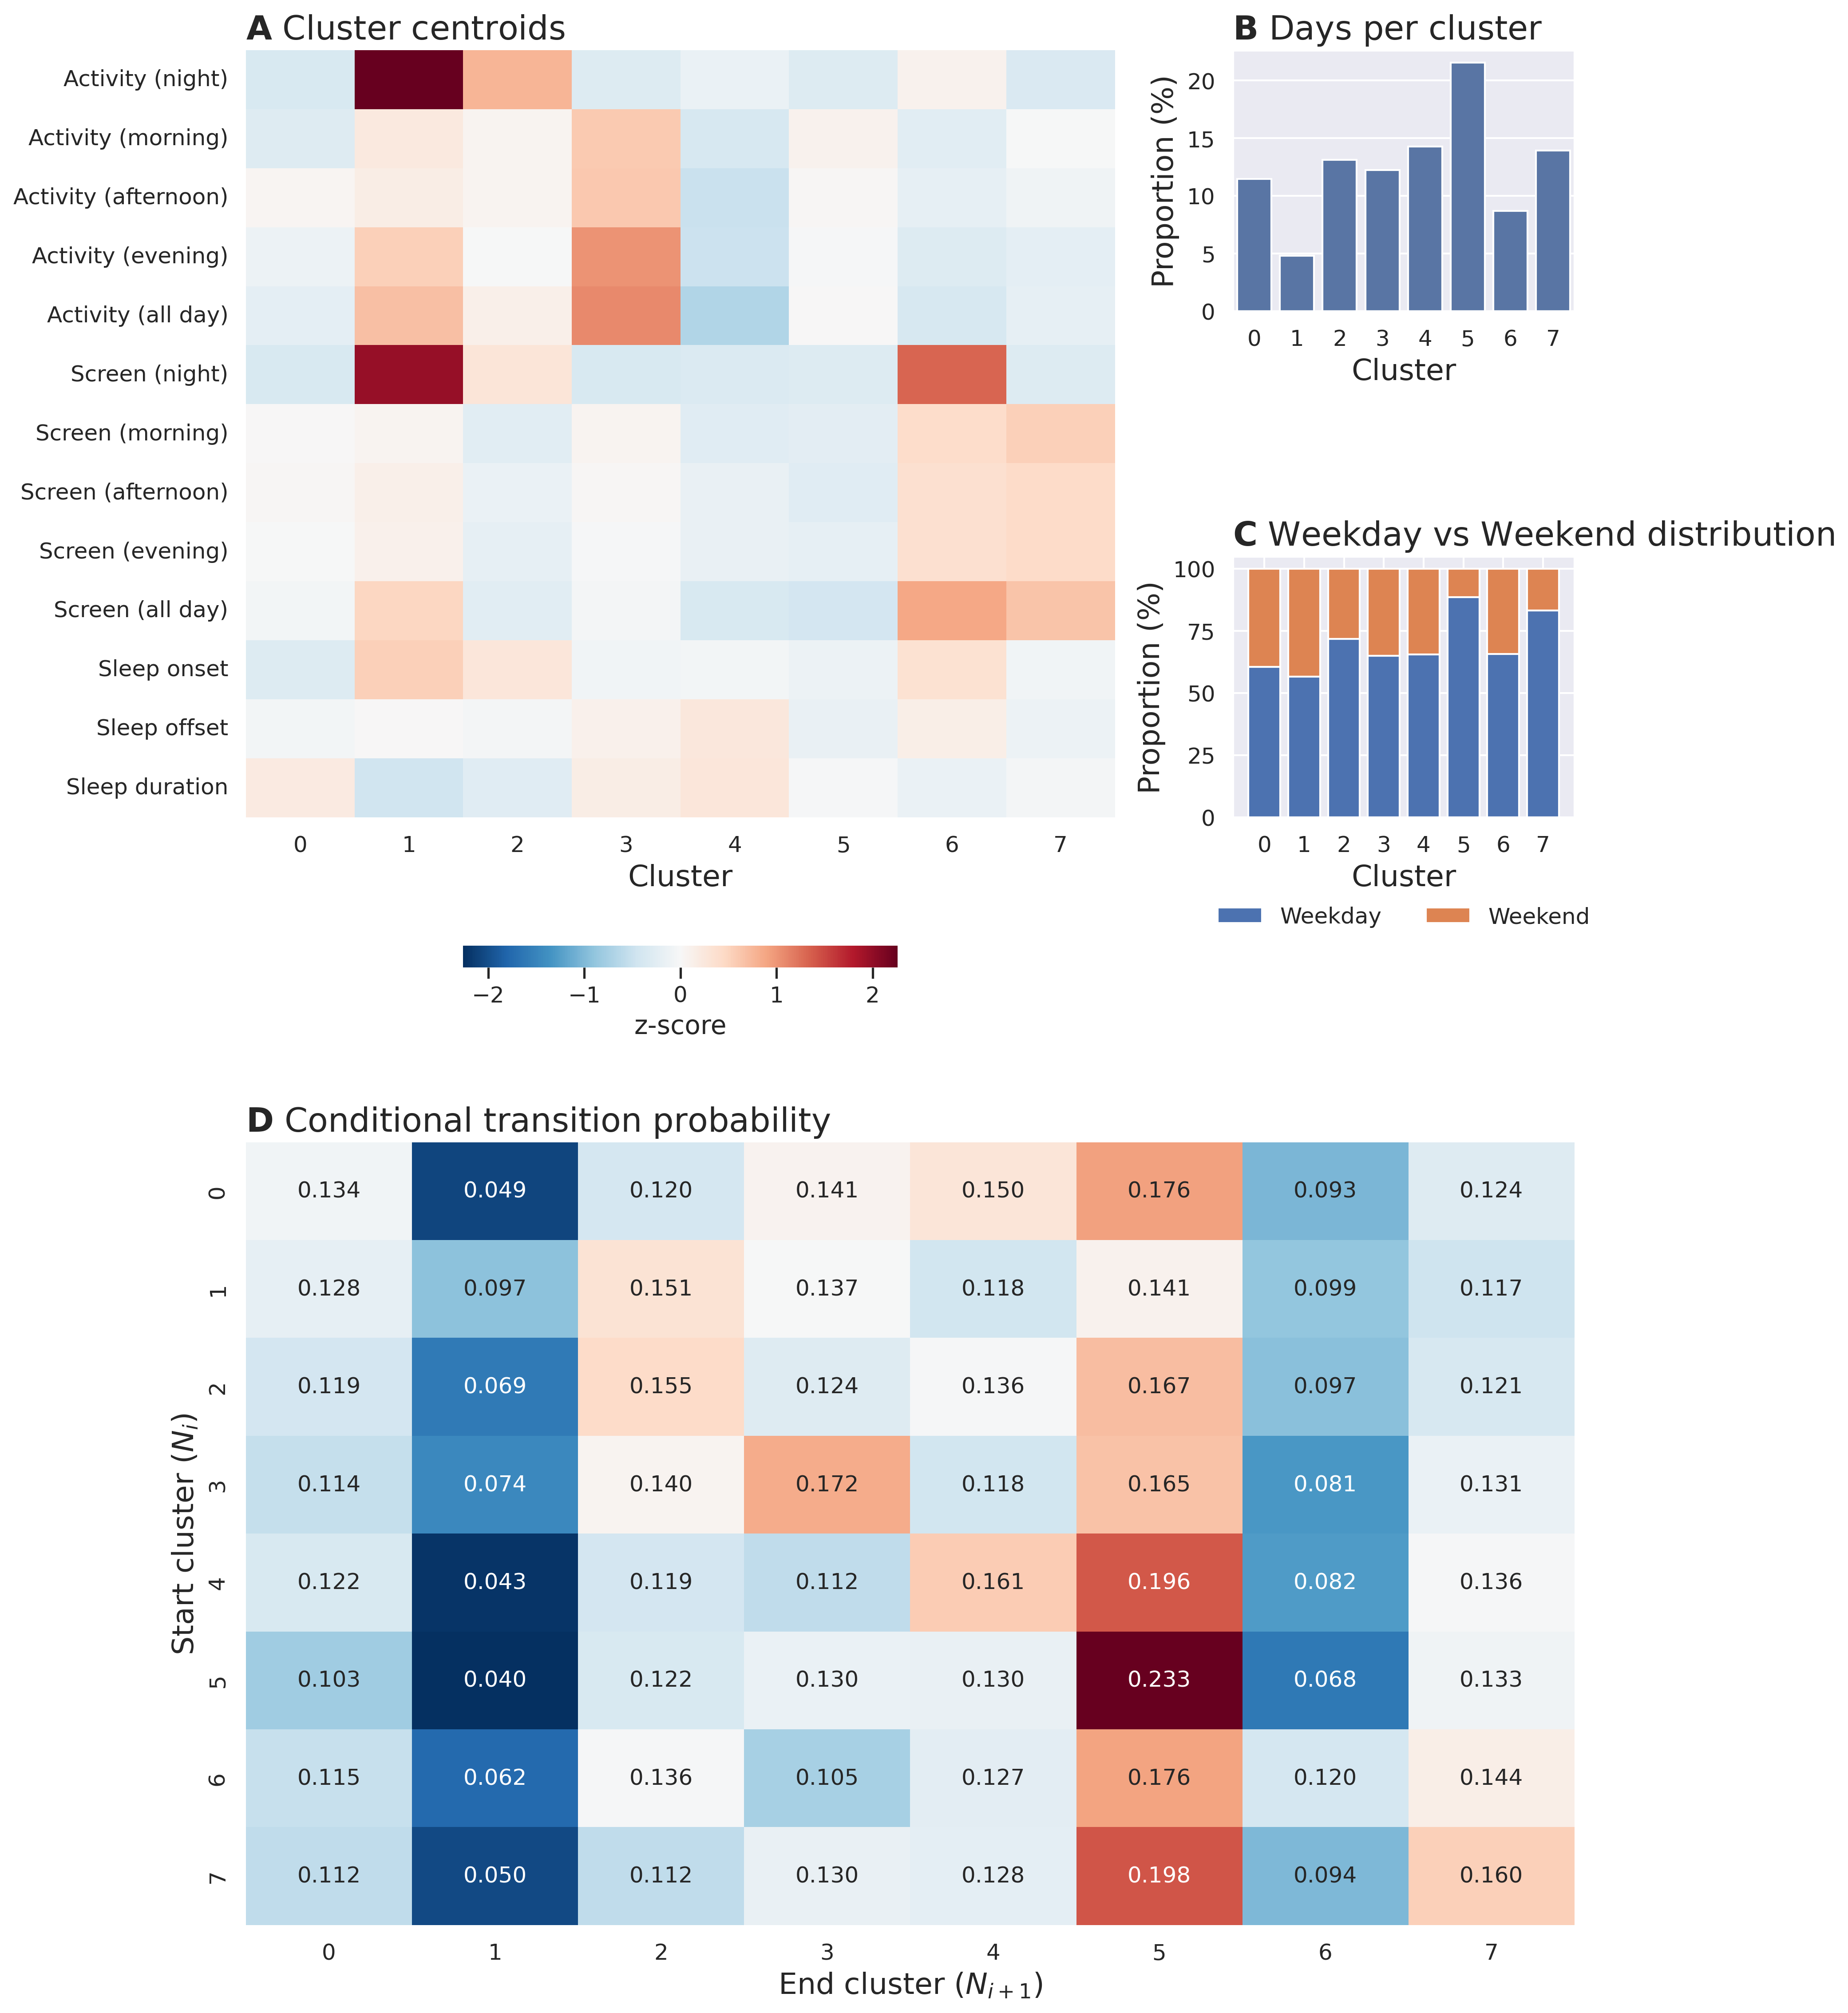
\includegraphics[width=1\linewidth]{figures/tesserae_summary.png}
    \caption{Cluster summary for Tesserae. (A) Cluster centroids: Heatmap showing the average standardized feature values (z-scores) for each behavioral feature within each cluster. Each feature’s z-score is computed per individual to reflect within-person deviations. Higher (red) and lower (blue) values represent positive and negative deviations from an individual’s mean, respectively. (B) Days per cluster: Histogram showing the distribution of all recorded days across clusters, aggregated across the study population. (C) Weekday–weekend distribution: Stacked bar plot depicting the proportion of weekdays (blue) and weekends (orange) within each cluster. Certain clusters exhibit a significant weekend skew, depicting leisure-oriented behaviours that emerge on non-working days. (D) Heatmap of adjacency matrix depicting the conditional transition probability between cluster pairs. Transition probabilities are computed and normalized per participant, then averaged across participants to obtain a population means. Higher values indicate more frequent transitions.}
    \label{fig:tesserae-cluster-summary}
\end{figure}

In Tesserae, the analysis included 592 participants and 106,172 person-days. The cluster centroids are shown in \autoref{fig:tesserae-cluster-summary}A, where each cell shows deviation from the within-person baseline. A single dominant cluster captures the most typical routine (see \autoref{fig:tesserae-cluster-summary}B): features lie near their mean with a small dip in screen use, consistent with a typical workday in this predominantly white-collar cohort. As illustrated in \autoref{fig:tesserae-cluster-summary}C, several smaller clusters also emerge that resemble weekend or holiday patterns, for exmample, slightly higher screen use and longer sleep (Cluster 4) or increase nocturnal mobility (Cluster 6). Notably, these weekend-like patterns naturally arise from the observations, given that temporal information was not provided during model fit. Cluster characteristics for MoMo-Mood and GLOBEM are reported in Appendix 2.

To test whether people remain in one routine or frequently switch among routine types, we modeled the day-to-day transitions between clusters. For each participant, we constructed a transition matrix \(P\) by counting the number of transitions from cluster \(i\) to cluster \(j\), then normalizing each row so that the probabilities sum to 1 (see \nameref{sec:methods}). Each cell \(P_{ij}\) represents the probability of transitioning from routine \(i\) to routine \(j\), with larger values indicating more frequent transitions. If individuals were strongly adapted to a specific routine, we would expect the diagonal entries \(P_{ii}\) - denoting self-transitions - to have the highest values. However, this was not the case. As shown in \autoref{fig:tesserae-cluster-summary}D, most routine clusters converged toward a dominant cluster. The transition probabilities were also diffuse and asymmetric, indicating that the likelihood of moving between clusters varies between individuals. We repeated the analysis on MoMo-Mood and GLOBEM and observed similar results, suggesting that these properties of routine transitions are consistent across different populations.

\subsection*{Persistence of individual's routine signature} \label{sec:results:signature_persistence}

Given between-person heterogeneity in time allocation across routine types, we posit that each individual exhibits a distinctive routine signature. Similar to the persistence of the social signature in communication \cite{saramaki2014persistence}, we hypothesize that this routine signature is also robust over time. For each participant and time segment, a \textit{routine signature} is defined as the vector of cluster proportions, sorted in descending order of frequency within that segment (\nameref{sec:methods}). We examined whether an individual’s routine is more similar to their own than to others’ by comparing the distributions of within-person distances \(d_{\text{self}}\) and between-person reference distances \(d_{\text{ref}}\) (see \autoref{fig:dself_dref}). For each participant \(i\), \(d_{\text{ref},i}\) was computed as the mean distance between \(i\)’s routine signature and those of all other participants, matched by time segment. To assess temporal stability, we determined minimum observation lengths and partitioned individual's records into two equal windows. For Tesserae and MoMo-Mood, we included participants with 270 days and split their data into two 135-day windows. For GLOBEM, given the shorter observation period, we included participants with 60 days and split into two 30-day windows.

Despite variability in total activity levels, individuals tended to allocate a large proportion of their time to a small number of routines, with the top two routines accounting for $(57.63 \pm 11.43)\%$ of total observations across all studies. This individuality was evident in the clear separation between participants’ signatures. In Tesserae (\(N=148\)), routine signatures were strongly persistent. Using JSD as distance metric, within-person distances were substantially smaller than between-person distances \dself{0.135}{0.041} vs. \dref{0.164}{0.026} (\dselfdrefpl{226.03}{-8.49}{10^{-3}}), indicating that individuals maintained highly distinctive routine patterns across time. A sanity check using cosine distance produced similar results, with \dself{0.031}{0.021} and \dref{0.055}{0.013} (\dselfdrefpl{246.83}{-11.69}{10^{-3}}).  

In MoMo-Mood (\(N=15\)), the patterns were similar despite the smaller sample size. Routine signatures again showed strong persistence, with JSD distances of \dself{0.164}{0.026} compared to reference distances \dref{0.222}{0.075} (\dselfdrefpl{29.99}{-12.13}{10^{-3}}). Robustness check using cosine distances also produced comparable results, with \dself{0.027}{0.026} and \dref{0.096}{0.035} (\dselfdrefp{27.8}{-6.21}{ 10^{-3}}). 

The same pattern emerged even when considering the shorter 30-day windows in GLOBEM. Again, within-person distances were smaller than between-person distances for both metrics: JSD \dself{0.201}{0.073} vs. \dref{0.218}{0.039} (\dselfdrefpl{293.31}{-2.85}{.005}) and cosine ( \dself{0.046}{0.042} vs. \dref{0.064}{ 0.031}, \dselfdrefp{345.9}{-4.58}{10^{-3}}). These results indicate that routine signatures are individual-specific, generalize across cohorts, and remain stable at shorter time scales.

\begin{figure}
    \centering
    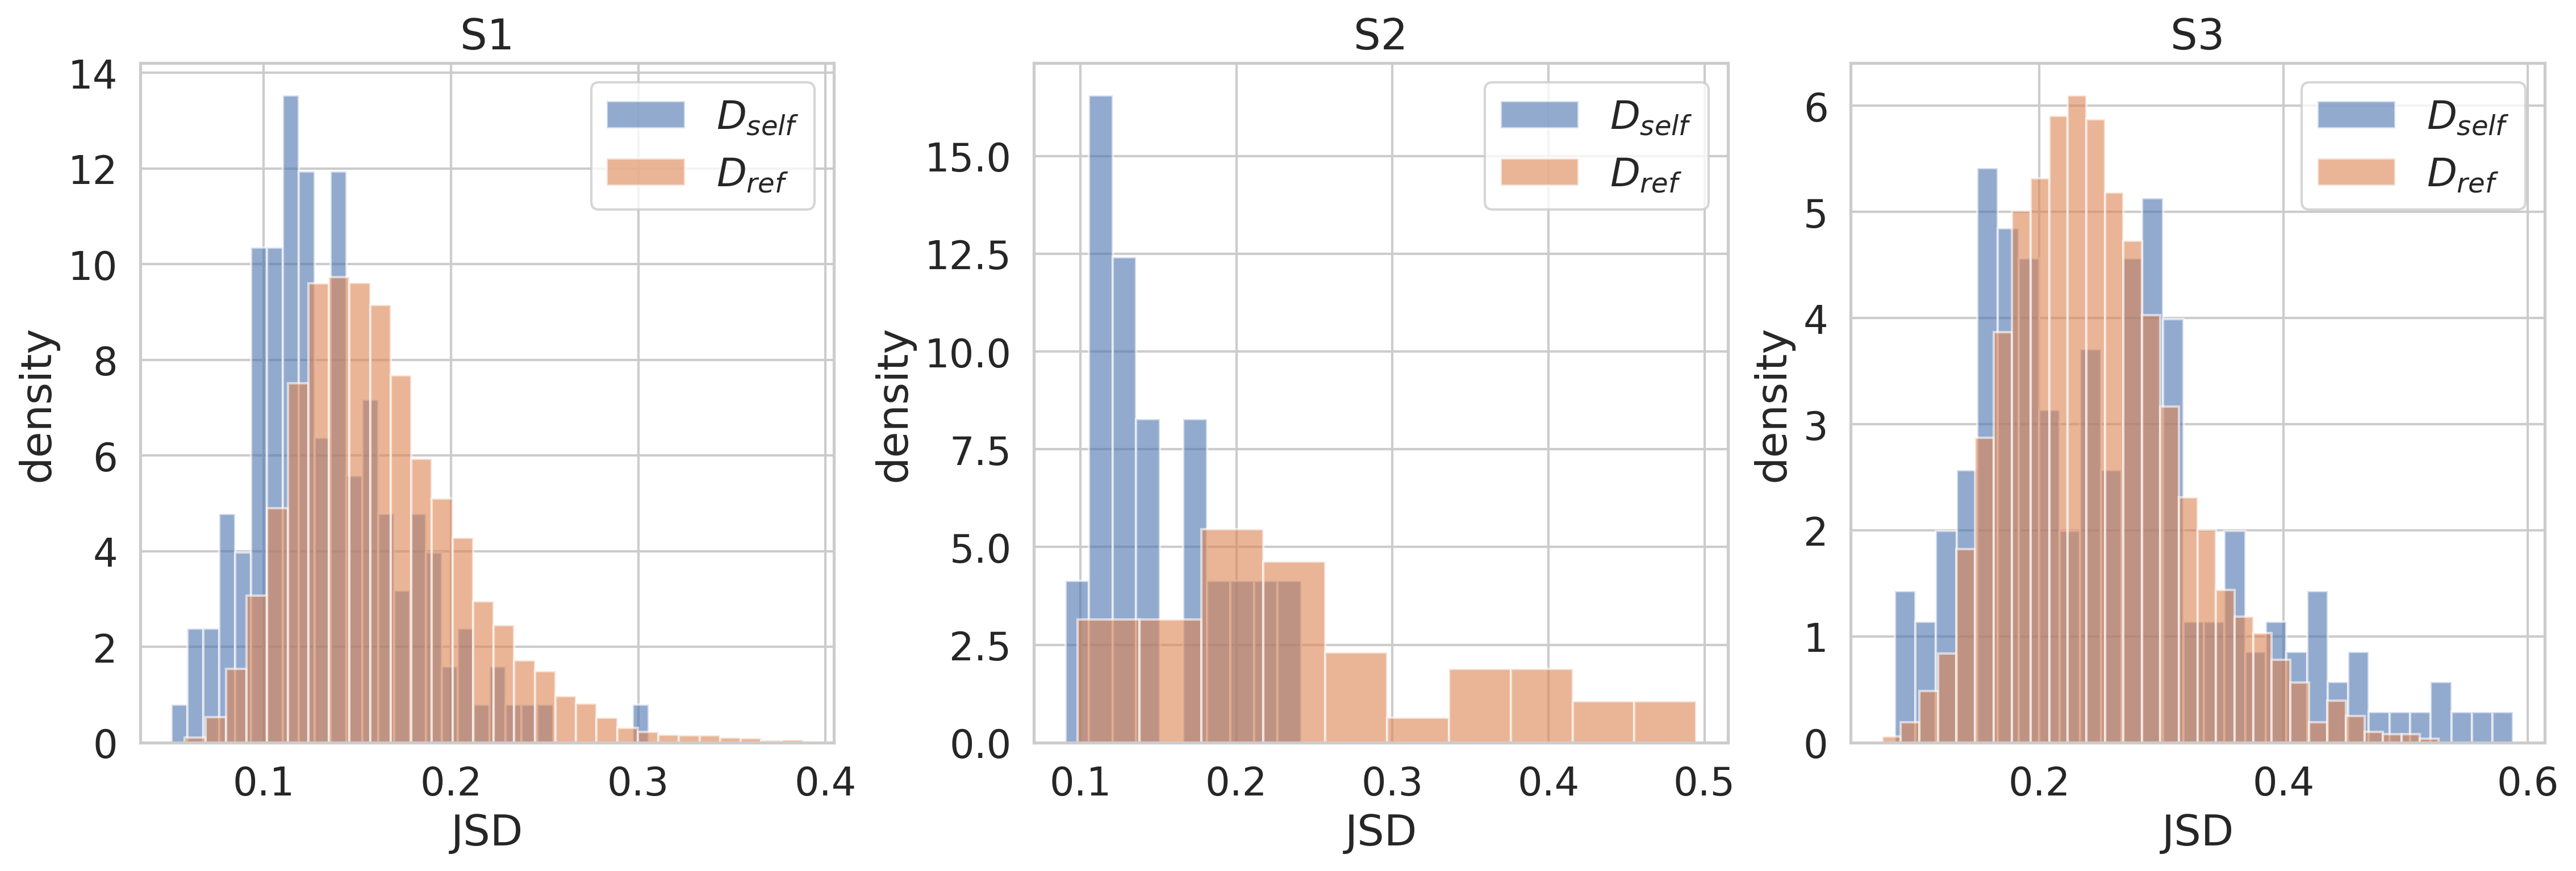
\includegraphics[width=1\linewidth]{figures/combined_dself_dref_ranked_jsd.png}
    \caption{Self-distance and reference-distance of routine signature across studies.}
    \label{fig:dself_dref}
\end{figure}

\subsection*{Transition between routines exhibits similar persistence}

Beyond individual-specific time allocation across routines, we hypothesized that each person’s transition dynamics between routines was also distinctive. In other words, people do not follow the same routine every day but instead switch between different latent routine clusters over time in unique ways. For example, one individual may frequently alternate between workday and weekend routines with minimal variability, whereas another may display irregular transitions across several distinct routine types.

To test this hypothesis, we first constructed a transition probability matrix 
\(\mathbf{P} \in \mathbb{R}^{K \times K}\) for each participant and segment, 
where \(K\) is the number of routine clusters. We define the transition signature of an individual as the mean row-wise 
distance between their transition matrices across consecutive segments: 
\(d_{\mathrm{self}} = 
D(\mathbf{P}^1, \mathbf{P}^{2}) \). Similarly, the reference distance of individual $i$ was computed by calculating the distance between each participant’s transition matrix with those of all other participants in the same segment, then averaged across 
segments: 
\(d_{\mathrm{ref}} = \frac{1}{2} (
D(\mathbf{P_i}^1, \mathbf{P_j}^{1}) + D(\mathbf{P_i}^2, \mathbf{P_j}^{2}))\)

\begin{figure}
    \centering
    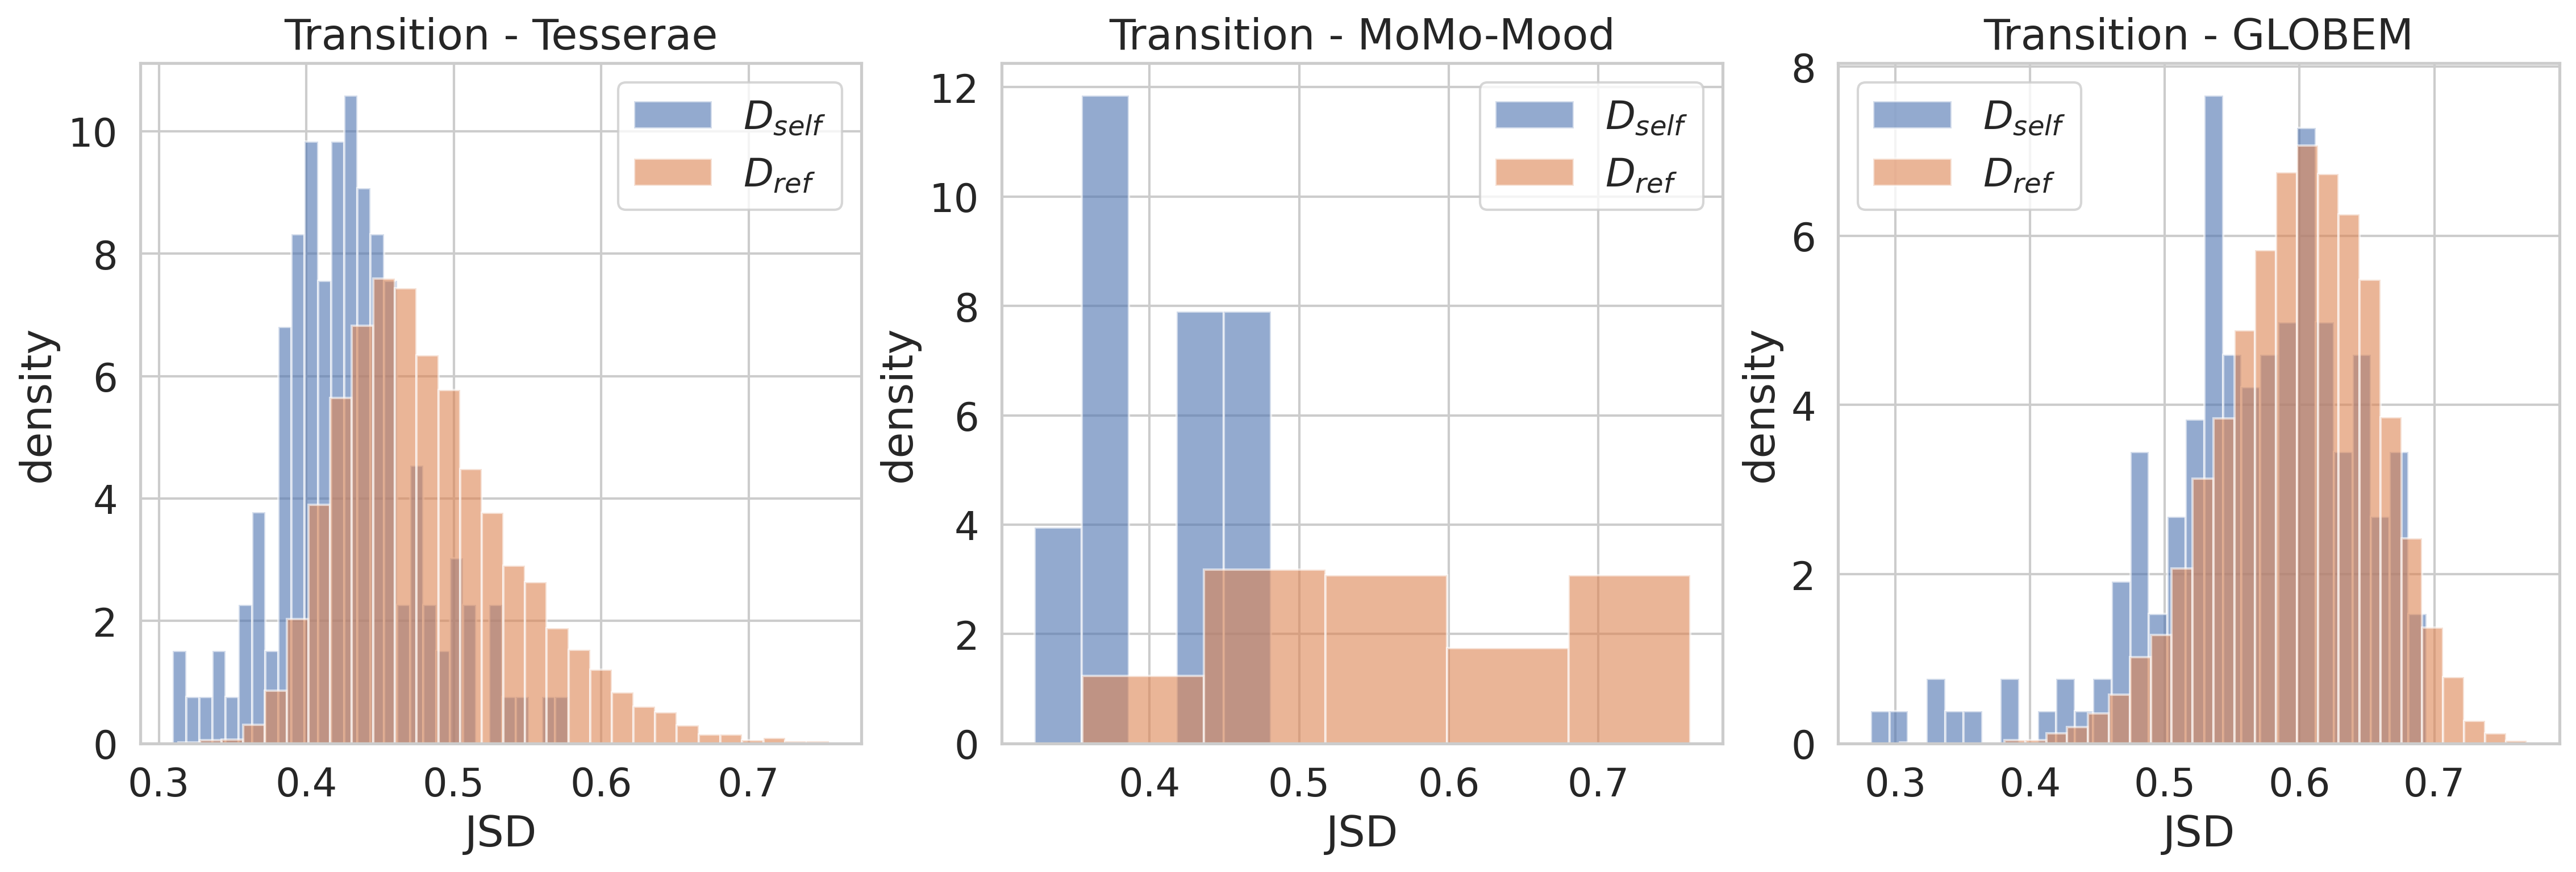
\includegraphics[width=1\linewidth]{figures/combined_transition_dself_dref_jsd.png}
    \caption{Transition signature}
    \label{fig:transition-signature}
\end{figure}

The within-person (\(d_{\text{self}}\)) and between-person (\(d_{\text{ref}}\)) distances between transition matrices are shown in \autoref{fig:transition-signature}. Their distributions resemble those observed for routine signature distances.
Across populations, transition signatures were temporally stable and person-specific with within-person distances consistently fell below between-person distances. In Tesserae, \dself{0.481}{0.044} < \dref{0.537}{0.029} (\dselfdrefp{255.65}{-12.86}{0.0}). In MoMo-Mood, the same pattern held, with \dself{0.458}{0.055} and \dref{0.600}{0.046} (\dselfdrefp{28.62}{-7.79}{0.0}). In GLOBEM, we again observed smaller within-person distances, \dself{0.565}{0.077} < \dref{0.598}{0.025} (\dselfdrefp{238.37}{-5.59}{0.0}). As with time allocation, transition patterns are also person-specific and stable, remaining more similar within individuals over time than between individuals.

\subsection*{Factors predicting persistence of routine signature}\label{sec3.3}

Prior work has linked sociodemographic factors \cite{luong2023impact, luong2024sleep, kulshrestha2021web} and personality traits \cite{centellegherPersonalityTraitsEgonetwork2017, alessandrettiUnderstandingInterplaySocial2018, amon2022flexibility} to the persistence of various types of routines.  Whether these relationships generalize to multifaceted routines remains unclear. We addressed this using two linear regression models: the first regressed routine-signature stability ($d_{\text{self}}$) on age, gender, and personality traits; the second used the same predictors to explain transition-signature stability ($d_{\text{self\_transition}}$). Due to difference in window size, we pooled participants in Tesserae and MoMo-Mood, and treated GLOBEM separately. For GLOBEM, we used a linear mixed-effects model to account for repeated measurements from participants from multiple waves.

\begin{table}[htbp]
\centering
\caption{OLS results for long-term $d_{\text{self}}$ and $d_{\text{self}}^{(\text{trans})}$.}
\label{tab:ols_signature_long}
\begin{tabular}{lcccccc}
\toprule
& \multicolumn{3}{c}{$d_{\text{self}}$} & \multicolumn{3}{c}{$d_{\text{self}}^{(\text{trans})}$} \\
\cmidrule(lr){2-4}\cmidrule(lr){5-7}
Predictors & Estimate & 95\% CI & $p$ & Estimate & 95\% CI & $p$ \\
\midrule
(Intercept)            & 0.018   & $-0.070$--$0.106$ & 0.686        & 0.321   & $0.228$--$0.414$ & \textbf{$<0.001$} \\
Extraversion           & 0.003   & $-0.008$--$0.013$ & 0.632        & 0.006   & $-0.005$--$0.017$ & 0.283 \\
Agreeableness          & $-0.005$& $-0.018$--$0.009$ & 0.477        & 0.001   & $-0.013$--$0.015$ & 0.930 \\
Conscientiousness      & 0.017   & $0.007$--$0.028$  & \textbf{0.001} & 0.013 & $0.002$--$0.025$  & \textbf{0.018} \\
Neuroticism            & 0.011   & $0.001$--$0.022$  & \textbf{0.039} & 0.010 & $-0.001$--$0.022$ & 0.080 \\
Openness               & 0.006   & $-0.005$--$0.018$ & 0.281        & 0.000   & $-0.012$--$0.013$ & 0.988 \\
Gender [Male]          & $-0.002$& $-0.019$--$0.015$ & 0.774        & $-0.000$& $-0.018$--$0.017$ & 0.958 \\
Age bin [$\ge 25$]     & 0.009   & $-0.016$--$0.034$ & 0.468        & 0.009   & $-0.016$--$0.035$ & 0.474 \\
\midrule
Observations           & \multicolumn{3}{c}{163} & \multicolumn{3}{c}{163} \\
$R^2$ / adj.\ $R^2$    & \multicolumn{3}{c}{0.098 / 0.057} & \multicolumn{3}{c}{0.064 / 0.022} \\
\bottomrule
\end{tabular}
\end{table}


\begin{table}[htbp]
\centering
\caption{Linear mixed-effects model results for short-term $d_{\text{self}}$ and $d_{\text{self}}^{(\text{trans})}$. }
\label{tab:lmer_short_signature_min}
\begin{tabular}{lcccccc}
\toprule
& \multicolumn{3}{c}{$d_{\text{self}}$} & \multicolumn{3}{c}{$d_{\text{self}}^{(\text{trans})}$} \\
\cmidrule(lr){2-4}\cmidrule(lr){5-7}
Predictors & Estimate & 95\% CI & $p$ & Estimate & 95\% CI & $p$ \\
\midrule
Extraversion           & 0.011   & $-0.001$--$0.023$ & 0.064 & $-0.006$ & $-0.018$--$0.005$ & 0.288 \\
Agreeableness          & $-0.003$& $-0.017$--$0.010$ & 0.625 & $-0.004$ & $-0.018$--$0.010$ & 0.546 \\
Conscientiousness      & 0.008   & $-0.004$--$0.021$ & 0.196 & 0.015    & $0.002$--$0.027$  & \textbf{0.025} \\
Neuroticism            & 0.002   & $-0.010$--$0.014$ & 0.713 & 0.010    & $-0.002$--$0.022$ & 0.100 \\
Openness               & $-0.004$& $-0.017$--$0.009$ & 0.540 & $-0.006$ & $-0.019$--$0.007$ & 0.389 \\
Gender [Male]          & 0.013   & $-0.011$--$0.037$ & 0.303 & $-0.002$ & $-0.025$--$0.022$ & 0.900 \\
Age                    & 0.006   & $-0.003$--$0.016$ & 0.191 & $-0.007$ & $-0.016$--$0.003$ & 0.171 \\
\midrule
Observations           & \multicolumn{3}{c}{186} & \multicolumn{3}{c}{186} \\
$R^2$ (marg./cond.)    & \multicolumn{3}{c}{0.045 / 0.123} & \multicolumn{3}{c}{0.069 / 0.069} \\
\bottomrule
\end{tabular}
\end{table}


 In all models, the persistence of routine was indifferent between demographic factors. For the short window models and transition signature, conscientiousness was positively associated with \(d_{\text{self}}^{(\text{trans})}\) (\(b=0.015\), 95\% CI \([0.002, 0.027]\), \(p=.025\)). For the long window models, the effects were clearer. Conscientiousness was positively associated with both \(d_{\text{self}}\) (\(b=0.017\), \([0.007, 0.028]\), \(p=.001\)) and \(d_{\text{self}}^{(\text{trans})}\) (\(b=0.013\), \([0.002, 0.025]\), \(p=.018\)), and neuroticism was positively associated with \(d_{\text{self}}\) (\(b=0.011\), \([0.001, 0.022]\), \(p=.039\)). Other factors, including extraversion, agreeableness, openness, gender, and age were not significant.

\section*{Discussions}\label{sec4}  

This work generalizes prior evidence on the persistence of human routines to a multifaceted setting. We introduce a framework that models routines as latent behavioral classes and quantifies persistence via each individual’s time allocation across these classes. Across three independent studies, individuals consistently allocated similar proportions of time to a small set of routines, yielding distinctive routine signatures. Beyond time allocation, day-to-day transition dynamics between routines were also person-specific, forming a complementary transition signature. Both signatures were distinctive and separable across individuals. Persistence was broadly similar across demographic groups (age, gender), but shown associations with personality traits such as conscientiousness.

To contextualize our findings, we draw comparisons with previous research on the stability of human behavior. The social signature, the tendency for individuals to distribute their communication efforts unevenly across social contacts, has been shown to remain stable over time within small cohorts \cite{saramaki2014persistence}, and later generalized to larger and more diverse populations \cite{heydari2018multichannel, iniguezUniversalPatternsEgocentric2023}. Similar forms of temporal persistence have also been observed in other routine modalities, including mobility patterns \cite{alessandrettiUnderstandingInterplaySocial2018, alessandretti2020scales} and online behaviors \cite{kulshrestha2021web, malmi2016you}. We extend these findings by integrating multiple behavioral domains and representing daily life as a distribution over latent routine classes. Individuals not only allocate time unevenly across a limited number of dominant routines, but also maintain a distinctive pattern of transitions between them. This former structure is similar to that of social signatures. Analogous to how most communication time is concentrated on a few close ties, much of one’s daily life is organized around a small set of core routines, such as weekday-weekend. For the latter, we find similarity to the stability of human mobility patterns in both physical and digital spaces. Individuals tend to follow consistent and repeatable paths, such as commuting to and from the same locations, or navigating through sequences of websites or applications. This pattern generalizes to daily routines more broadly: people transition between behavioral states in structured and habitual ways, thus forming individualized transition routines.

Our approach starts from a simple premise: complex, multimodal behaviour can be captured by a small set of latent routine classes \cite{eagleEigenbehaviorsIdentifyingStructure2009a,aledavood2022quantifying,zhou2022predicting}. Although the approach is unsupervised, the principle findings are robust to the number of components and distance metrics: people spend most of their time in a few dominant routines, and the resulting signatures remain stable over time. This mirrors regularities in other domains—people repeatedly visit a limited set of places \cite{alessandretti2020scales} and use familiar apps \cite{sekaraTemporalCulturalLimits2021}. The distinctiveness of these signatures implies re-identification risk. Because individuals are distinguishable even over short windows, a natural next step is to quantify data sufficiency: how many days are needed to reach reliable discrimination and to examine heterogeneity in this requirement.

Our study has several limitations, both in the data's properties and methodology. On the data side, although we considered multiple routine modalities, common routines like location and communication were not included due to missingness and sparsity of features. GPS signals showed substantial missingness across datasets, so we excluded location features to avoid biased estimates. Communication activity was logged only via calls and SMS. Without app-based messaging, the communication feature space was sparse and zero-inflated. As a result, clustering on these variables tended to produce a dominant “no communication” cluster that mainly separated participants with any call/SMS activity from those with none. On the methodology side, our clustering approach are also limited in many ways. While the number of latent classes was selected via model selection, the model remains unsupervised in nature, meaning that the resulting clusters can vary between population or carry different meanings, and making interpretation hard. Furthermore, by clustering via a bag-of-days method, we ignored the sequential temporal order of routines. Even so, we observed a clear weekday–weekend split among clusters, indicating strong periodicity that emerges even without explicit temporal modeling. Future work can consider temporal dependencies via appropriate methods such as Markov model \cite{liuIntraindividualPhenotypingDepression2024, leaningUncoveringSocialStates2025}.

\section*{Methods}\label{sec:methods}  

\subsection*{Study description}\label{sec:methods:study_desc}  

We used datasets gathered from three multisensor, longitudinal studies. An overview of feature processing and bulding of routine signature is presented in \autoref{fig:routine-sig-workflow}.

\textbf{Tesserae.} The Tesserae study recruited 757 information workers across the United States \cite{mattingly2019tesserae}. Participants were provided a Garmin Vivosmart 3 wristband to monitor mobility, heart rate, sleep, and calories. Additionally, participants installed a custom smartphone app that passively tracked screen activity, data usage, charging behavior, location, and other phone states.

\textbf{MoMo-Mood.} The MoMo-Mood study involved patients diagnosed with major depressive episodes, including Major Depressive Disorder (MDD), Bipolar Disorder (BD), and Borderline Personality Disorder (BPD), as well as healthy controls (HC). The study recruited a total of 164 participants from Finland: 133 patients and 31 HCs \cite{aledavood2025multimodal}. Data were collected over a one-year period from smartphones using the AWARE platform \cite{ferreiraAWAREMobileContext2015}, which tracked screen activity, calls and SMS, charging behavior, location, and accelerometer.

\textbf{GLOBEM.} The GLOBEM study procured a multi-year passive sensing datasets of over 700 user-years of data from 497 unique college students \cite{xu2022globem}. Longitudinal data, including location, phone usage, calls, Bluetooth, mobility, and sleep behavior, were collected from a mobile app and fitness trackers. The study spanned four years, with data collection occurring over a 10-week period each year, primarily during the spring semester. 

\subsection*{Features extraction and Preprocessing} \label{sec:methods:features_extraction}  

\textbf{Sleep.} Bed time, wake time, and sleep duration were collected directly from Garmin (Tesserae) and Fitbit (GLOBEM) fitness trackers. In MoMo-Mood, due to the lack of wearable devices, sleep was estimated using phone lock/unlock status, with the longest lock episode considered sleep. To assess the validity of this proxy, sleep parameters from the same participants were compared to those derived from actigraphy during a two-week validation phase. The comparison revealed a slight bias but demonstrated adequate correlation between the two methods.

\textbf{Mobility.} This routine was measured using step count data collected from fitness trackers in the Tesserae and GLOBEM studies. In MoMo-Mood, due to the lack of fitness trackers, mobility was estimated using the standard deviation of the accelerometer magnitude \cite{ravi2005activity}. Accelerometer readings displayed a clear 24-hour rhythm, consisting of higher activity levels during the day, a peak around a specific hour, and a gradual decline toward the end of the day. To capture daily activities pattern, activity readings were aggregated into four 6-hour time bins as proxy for four parts of the day (night, morning, afternoon, evening). A daily average value was also computed.

\textbf{Device usage.} The hourly duration of screen use episodes was extracted. Similar to mobility, daily rhythms for screen usage were constructed by aggregating the hourly measures into 4-hour bins. 

\textbf{Demographics and personality traits.} Baseline demographics (age, gender, occupation) were recorded at enrollment. In Tesserae, age was available only in aggregated bins; to ensure comparability, we applied the same binning across all studies: \(<\!25\), \(25\text{--}34\), \(35\text{--}44\), \(45\text{--}54\), and \(55\text{--}64\). Personality traits were assessed with the BFI-10 questionnaire \cite{rammstedt2007measuring} in Tesserae and GLOBEM and the NEO-60 questionnaire \cite{costa1992neo} in MoMo-Mood. Because Tesserae reported personality traits as aggregate scores on a 1–5 scale, we linearly rescaled the MoMo-Mood and GLOBEM trait scores to the same $[1,5]$ range for cross-study comparability.

\textbf{Exclusion and normalization}: The records from the first and last day of any user were excluded due to high likelihood of data incompleteness. We excluded participants with fewer than 14 days of data for clustering task. Any day with missing data on device usage, mobility, or sleep were excluded. Each feature was z-normalized within participants, allowing the model to focus on intra-individual variability. The resulting daily vector contained 13 features (see \autoref{tab:features_list}). Dimensionality reduction was not performed because the feature space is reasonably small and bnm  retaining the original variables preserves interpretability of the subsequent clustering results.

\begin{table}[ht]
    \centering
    \begin{tabular}{ll}
        \toprule
        \textbf{Routine} & \textbf{Features} \\
        \midrule
        mobility & Step count (MoMo-Mood, GLOBEM); accelerometer (Tesserae): daily average + MAEN \\
        Sleep             & bedtime, wake time, sleep duration \\
        Device usage      & Screen usage duration: daily average + MAEN \\
        \bottomrule
    \end{tabular}
    \caption{List of daily behavioral features, grouped by routine domain. MAEN = Morning, Afternoon, Evening, Night segments.}
    \label{tab:features_list}
\end{table}

\subsection*{Building routine cluster using GMM}\label{sec:methods:building_cluster}

For each participant, we formed an $M \times N$ matrix of daily features ($N$ features over $M$ days) and fit a $K$-component Gaussian Mixture Model (GMM). The $K$ multivariate Gaussian components (means $\boldsymbol{\mu}_k$, covariances $\boldsymbol{\Sigma}_k$, weights $\pi_k$) represent latent routines. This approach captures both the mean behavioral profile (via the components' mean) and the variability and correlation among features (via the covariance matrices).
Compared to clustering methods like K-Means, GMM offers greater flexibility. First, GMM supports soft clustering, meaning each day is assigned to multiple routine types with varying probabilities, modelling the transition nature of human behavior. Second, each GMM component can be parameterized by the full covariance structure, which captures the interdependencies between routines. For instance, increased phone activity late at night may correlate with delayed bedtime. Third, probabilistic assignments of cluster enable detection of anomalous routines, i.e. days which do not fit into any type of routines.

GMM has two main hyper-parameters: the number of components \(k\) and the covariance type (full, tied, diagonal, or spherical). 
Model selection was based on the Bayesian Information Criterion (BIC), with lower values indicating better fit. For model with full covariance matrix, we quantified cluster separation by computing all pair-wise Bhattacharyya distances. 
For two multivariate Gaussian clusters \(p_1 \sim \mathcal{N}(\boldsymbol{\mu}_1, \boldsymbol{\Sigma}_1)\) and \(p_2 \sim \mathcal{N}(\boldsymbol{\mu}_2, \boldsymbol{\Sigma}_2)\), the Bhattacharyya distance is

\[
D_B(p_1,p_2)
    = \frac{1}{8}\,
      (\boldsymbol{\mu}_1 - \boldsymbol{\mu}_2)^{\mathsf T}
      \boldsymbol{\Sigma}^{-1}
      (\boldsymbol{\mu}_1 - \boldsymbol{\mu}_2)
      + \frac{1}{2}\,
        \ln\!\left(
          \frac{\det\boldsymbol{\Sigma}}
               {\sqrt{\det\boldsymbol{\Sigma}_1\,\det\boldsymbol{\Sigma}_2}}
        \right),
\]

where
\[
\boldsymbol{\Sigma} = \frac{1}{2} \left( \boldsymbol{\Sigma}_1 + \boldsymbol{\Sigma}_2 \right)
\]
is the average covariance matrix, and \(\boldsymbol{\mu}_1,\boldsymbol{\mu}_2\) are the cluster mean vectors. Larger values indicate better separation between clusters.

We assigned each day to one of the resulting components. This clustering process was carried out independently for each study. For GLOBEM, the dataset spanned multiple academic years, so we fitted the clustering model separately for each year (semester). The tuning process is detailed in Appendix 1.

\subsection*{Routine signature}\label{sec:methods:signature}  

Social signature describes how individuals persistently distribute their communication efforts across their social contacts \cite{saramaki2014persistence}. We extended this concept by introducing the notion of a routine signature—the characteristic way in which individuals distribute their time across recurring patterns of daily behavior. Our concept aims to capture the persistence in the way individuals structure their daily lives across different types of routines.

For each participant, we represented every day in terms of behavioral features and assigned GMM cluster. Then, we summarized how often each cluster occurred for that participant by counting the number of days assigned to each cluster. To obtain a comparable distribution across individuals, these counts were normalized into proportions, giving the fraction of the participant’s days that belonged to each cluster.  

The clusters were then ranked in descending order of frequency (rank 1 = the most common cluster for that participant). 
The resulting vector of ranked proportions constitutes the \textit{routine signature} of that individual:

\begin{equation}
    \sigma_i = \left(
    \frac{n_{i1}}{\sum_j n_{ij}},\;
    \frac{n_{i2}}{\sum_j n_{ij}},\;
    \ldots,\;
    \frac{n_{ik_i}}{\sum_j n_{ij}}
    \right),
\end{equation}

where \(n_{ij}\) is the number of days participant \(i\) spent in cluster \(j\), and the elements are ordered so that \(\sigma_{i1} \geq \sigma_{i2} \geq \dots\).  

Intuitively, the routine signature reflects the individual pattern of time allocation across latent routines, independent of the cluster labels themselves. In line with the concept of social signatures, we expect this pattern to persist over time.

\begin{figure}[!htbp]
    \centering
    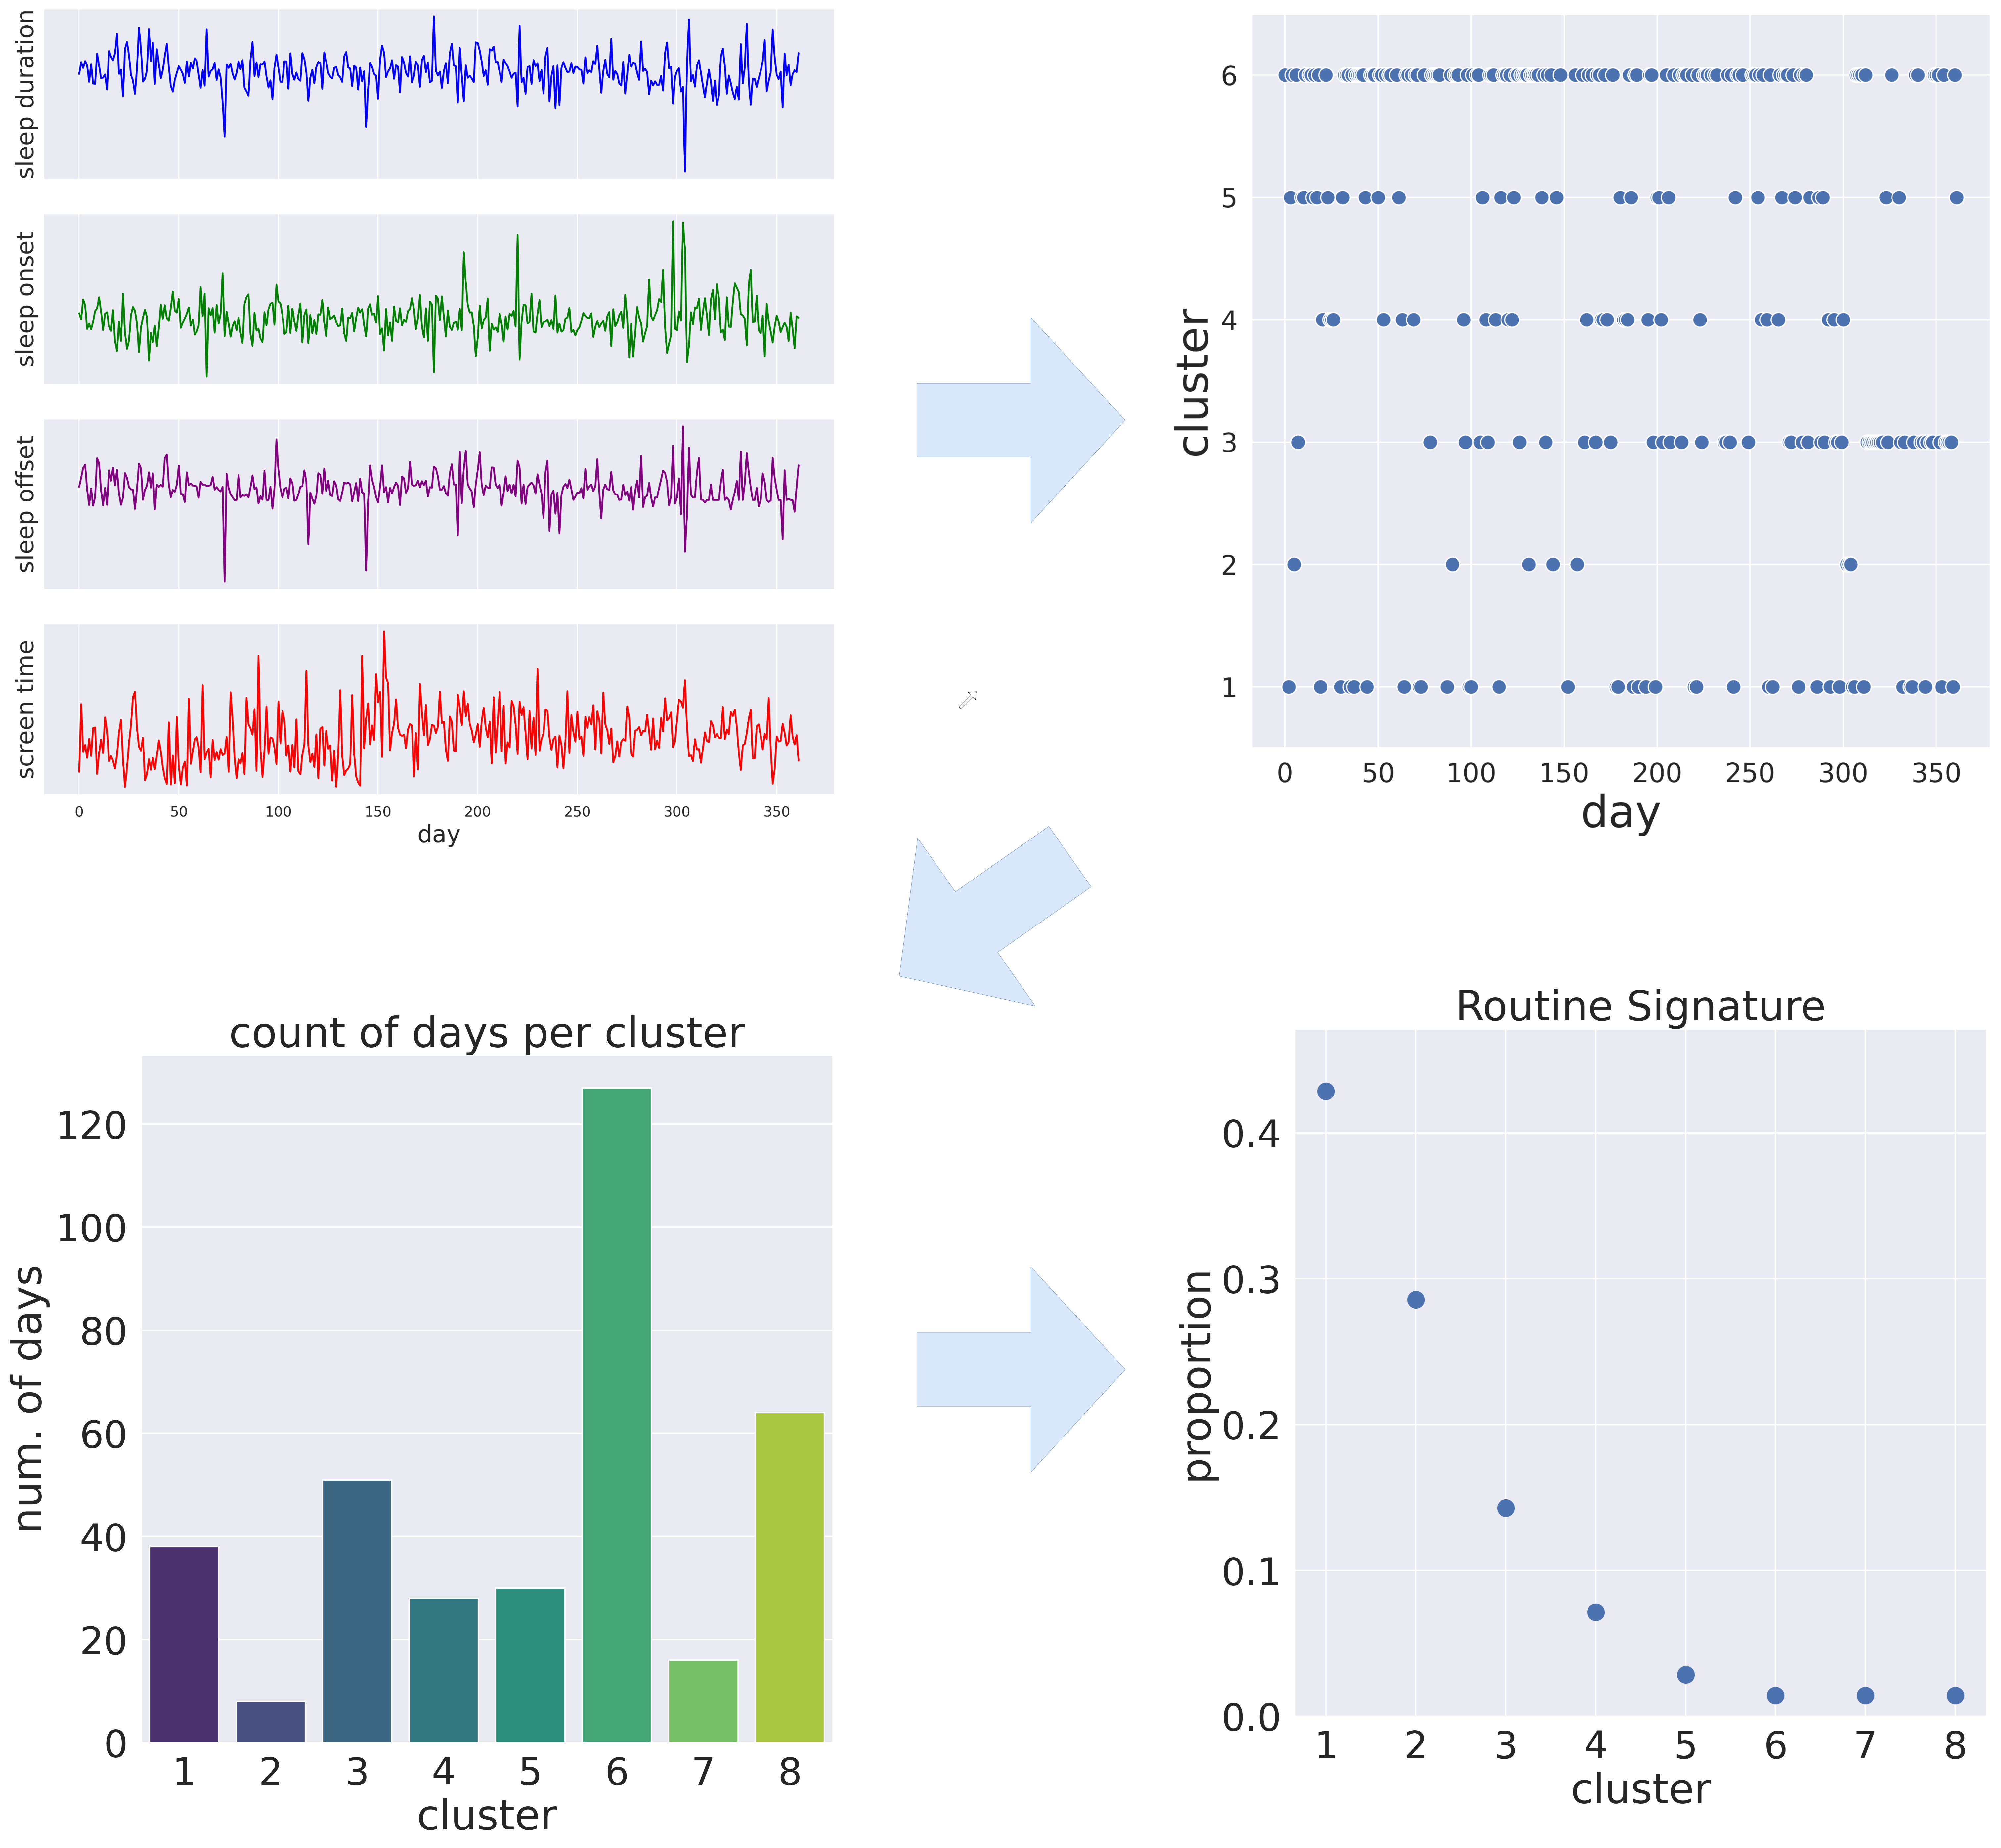
\includegraphics[width=\textwidth]{figures/digi-schema.png}
    \caption{Schematic description of routine signature. (A) Raw data capturing each person-day’s routine (e.g., sleep times, screen use, activity levels).
(B) Gaussian Mixture Model (GMM) fitted on the pooled person-day assigns each day to one of the routine clusters.
(C) For each individual, the number of days falling into each GMM‐defined cluster is computed and clusters are ranked by descending day‐counts.
(D) These counts are converted into proportions, giving each person’s routine signature.}
    \label{fig:routine-sig-workflow}
\end{figure}

\subsection*{Persistence of routine signatures}\label{sec:methods:signature_persistence}  

To quantify the persistence of routine signature, we examine how robust a person maintain the time allocated to their routine over time. For each person, the data was divided into 3 equal time segments. Due to the difference fin study design, the segmenting strategy was done differently for each dataset. For Tesserae and MoMo-Mood, each segment consisted of 90 days of data, hence we retained users with at least 270 data days. For GLOBEM, each segment equals to each wave, i.e 10 weeks of data, and we retained the users that participated in at least 2 waves of the study. The persistence of routine was defined as the distance between the routine signatures in consecutive time segments, using the Jensen-Shannon divergence (JSD) \cite{lin1991divergence}:

\begin{equation}
JSD(\sigma_1, \sigma_2) = H(\frac{\sigma_1 + \sigma_2}{2}) - \frac{1}{2}[H(\sigma_1) + H(\sigma_2)]
\end{equation}

where $\sigma_1$ and $\sigma_1$ are the social signatures defined in Eq. 1, and $H(\sigma)$ is the Shannon entropy of $\sigma$.

To determine how well one maintains their routines over time, we define $d_{self} =  d_{12}$. We validate individual's persistence against the population, by computing the reference distance $d_{ref} = \frac{1}{2}* (d_{i1j1} + d_{i2j2} )$. That is, we compute the routine signature in each time split of individual $i$ against that from the same time split of individual $j$.




%%===========================================================================================%%
%% If you are submitting to one of the Nature Portfolio journals, using the eJP submission   %%
%% system, please include the references within the manuscript file itself. You may do this  %%
%% by copying the reference list from your .bbl file, paste it into the main manuscript .tex %%
%% file, and delete the associated \verb+\bibliography+ commands.                            %%
%%===========================================================================================%%

\bibliography{sn-bibliography}% common bib file
%% if required, the content of .bbl file can be included here once bbl is generated
%%\input sn-article.bbl

\clearpage
% Uncomment to include appendix
% Preamble additions (recommended)
% \usepackage{graphicx}
% \usepackage{subcaption}
% \usepackage{placeins}   % for \FloatBarrier
% \usepackage{float}      % if you want [H] placement (optional)

\section{Appendices}

\begin{appendices}

% ---------- A: GMM model tuning ----------
\clearpage                    % start this appendix section on a new page
\section{GMM model tuning}

Model tuning across all cohorts favored Gaussian mixtures with full covariance matrices, yielding lower Bayesian Information Criterion (BIC; lower is better) and higher average Bhattacharyya distances between components (greater separation). Performance improved up to \(K=8\) and then showed diminishing returns, so we fixed \(K=8\) for the main analyses. All principal findings were confirmed in a sensitivity analysis with \(K \in \{6,\ldots,11\}\).


\begin{figure}[p]
  \centering
  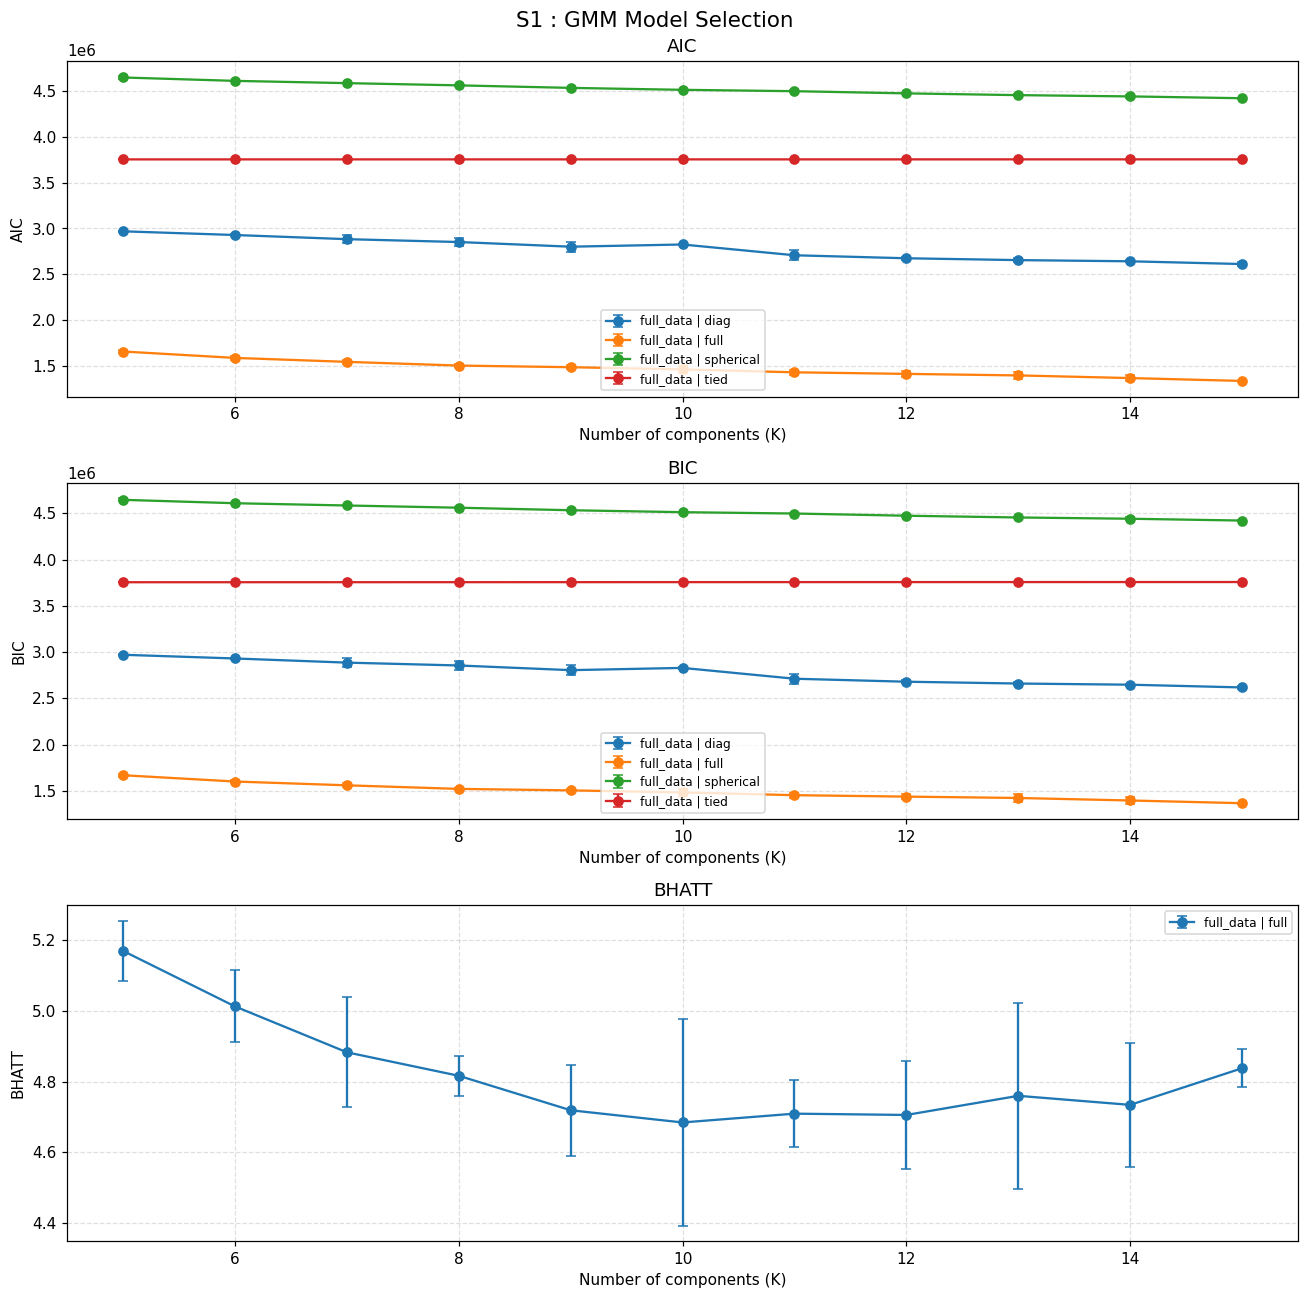
\includegraphics[width=\linewidth]{figures/appendix/tesserae_gmm_model_selection.png}
  \caption{Tesserae: Model selection}
  \label{fig:tesserae_model_selection}
\end{figure}

\begin{figure}[p]
  \centering
  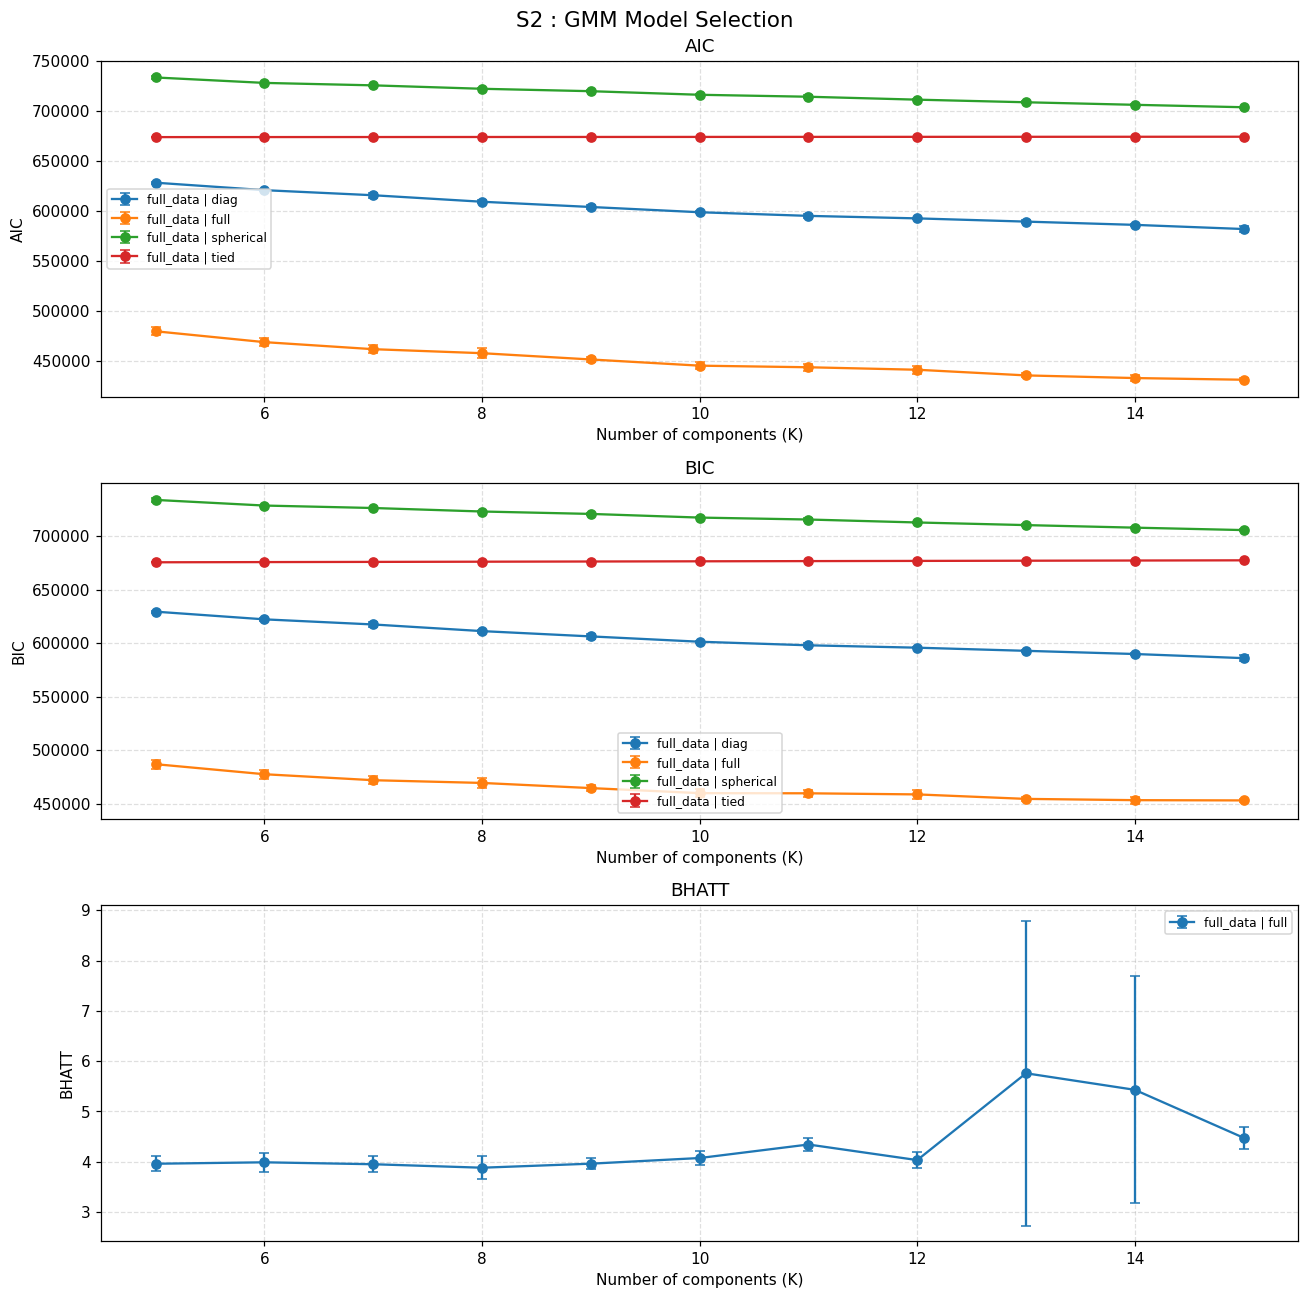
\includegraphics[width=\linewidth]{figures/appendix/momo_gmm_model_selection.png}
  \caption{MoMo-Mood: Model selection}
  \label{fig:momo_gmm_model_selection}
\end{figure}

\begin{figure}[p]
  \centering
  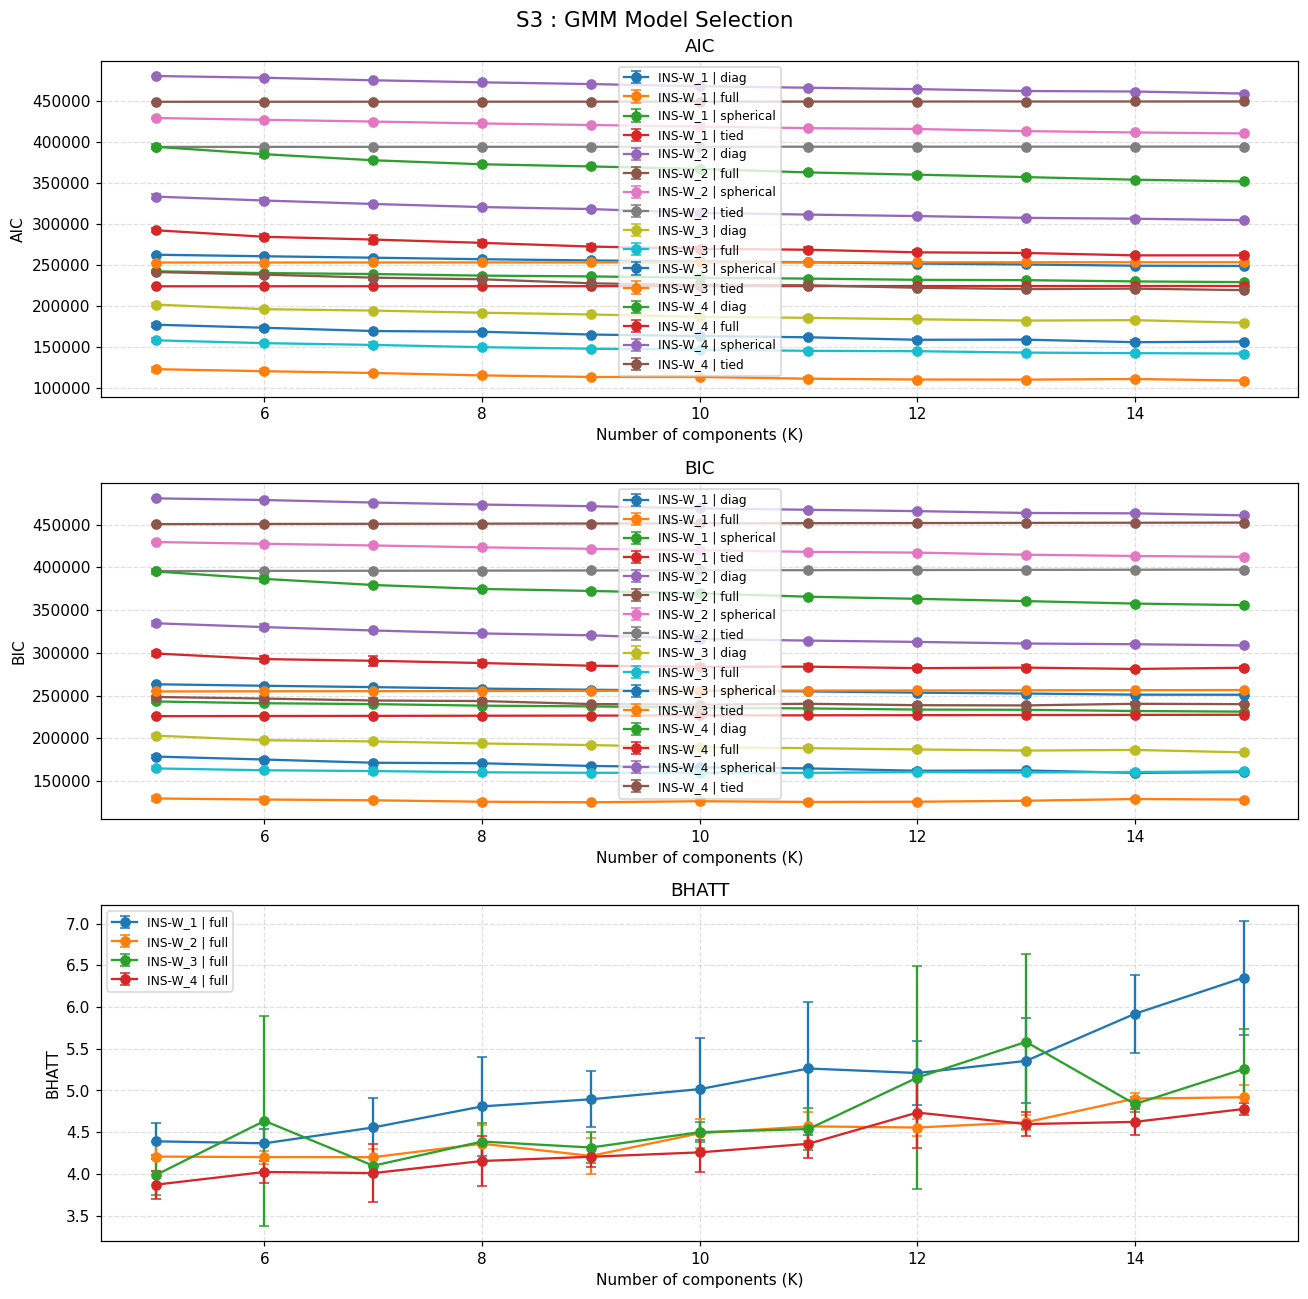
\includegraphics[width=\linewidth]{figures/appendix/globem_gmm_model_selection.png}
  \caption{GLOBEM: Model selection}
  \label{fig:globem_gmm_model_selection}
\end{figure}

\FloatBarrier                 % ensure these floats don’t spill into the next section

% ---------- B: Cluster properties ----------
\clearpage
\section{Cluster properties of MoMo-Mood and GLOBEM}

\autoref{fig:momo_centroid_summary} and \autoref{fig:globem_centroids} describe the cluster characteristics of the MoMo-Mood and GLOBEM studies, respectively. Across both datasets, a few dominant clusters account for the majority of time, while other clusters reflect free day routines, for example, elevated nightly activity or increased nighttime screen use.

\begin{figure}[p]
  \centering
  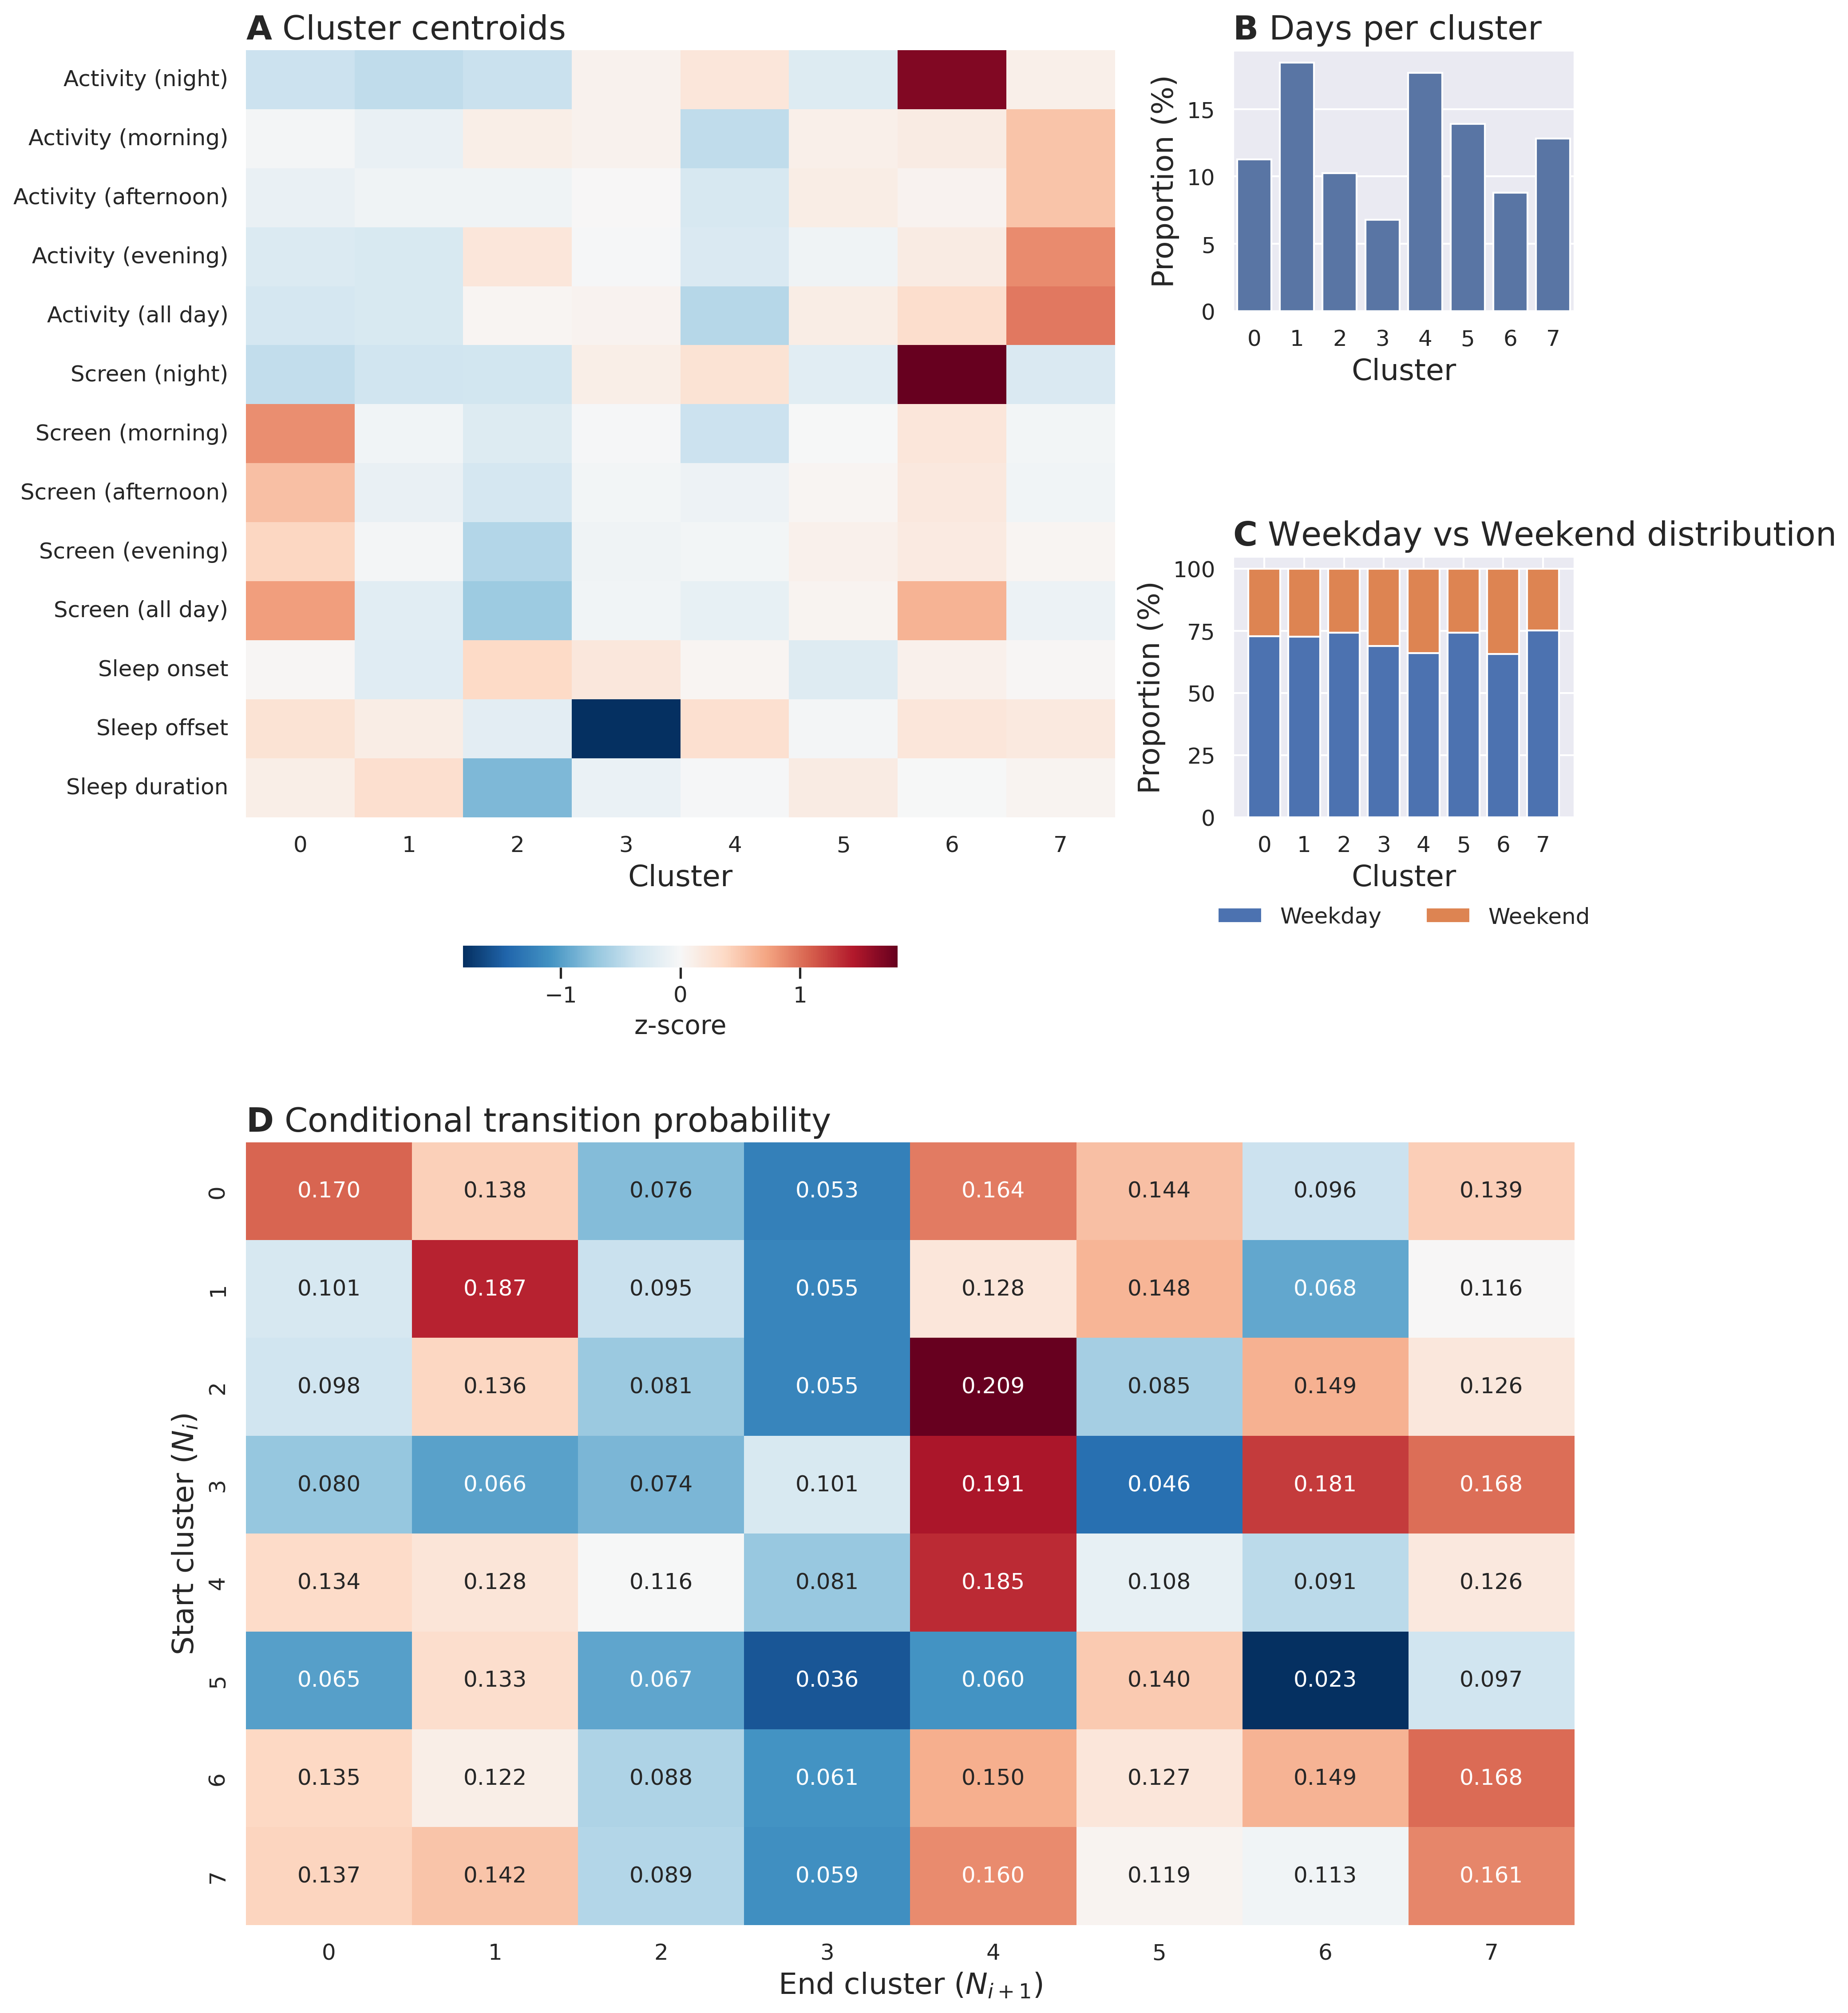
\includegraphics[width=\linewidth]{figures/appendix/momo_summary.png}
  \caption{MoMo-Mood: Cluster centroid characteristics}
  \label{fig:momo_centroid_summary}
\end{figure}

% 2x2 subfigures for GLOBEM centroid characteristics (example filenames 1–4)
\begin{figure}[p]
  \centering

  \begin{subfigure}[t]{0.485\textwidth}
    \centering
    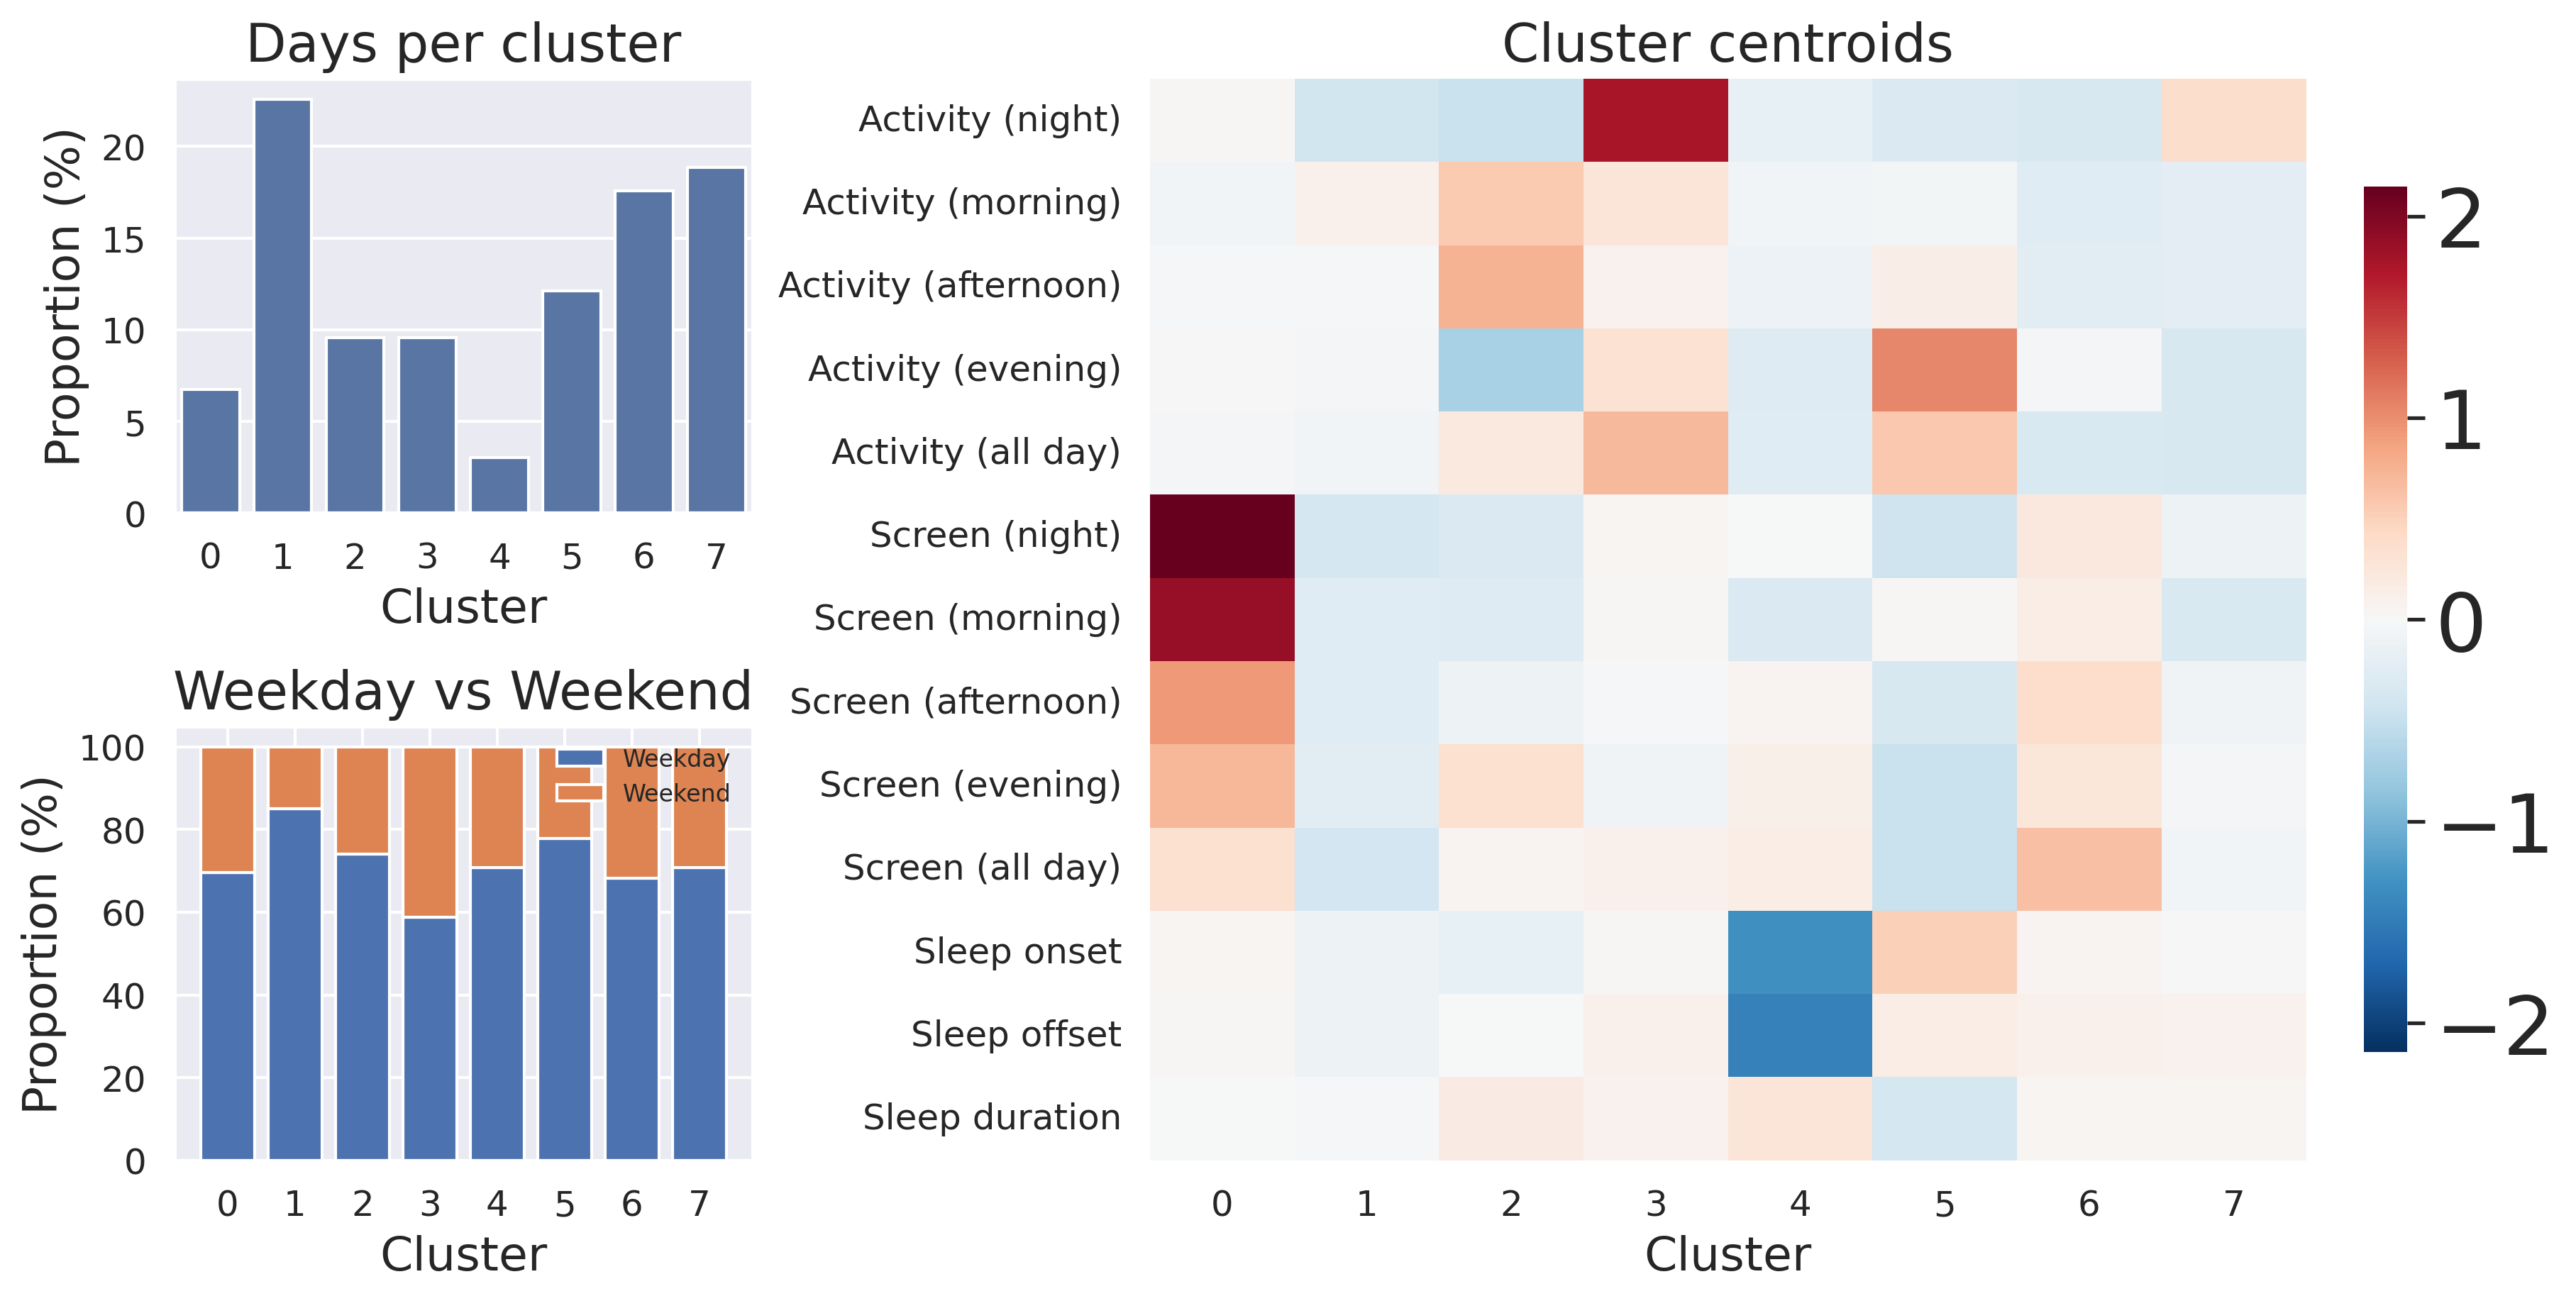
\includegraphics[width=\linewidth]{figures/appendix/globem_INS-W_1_summary.png}
    \caption{Cluster 1}
    \label{fig:globem_centroids_a}
  \end{subfigure}\hfill
  \begin{subfigure}[t]{0.485\textwidth}
    \centering
    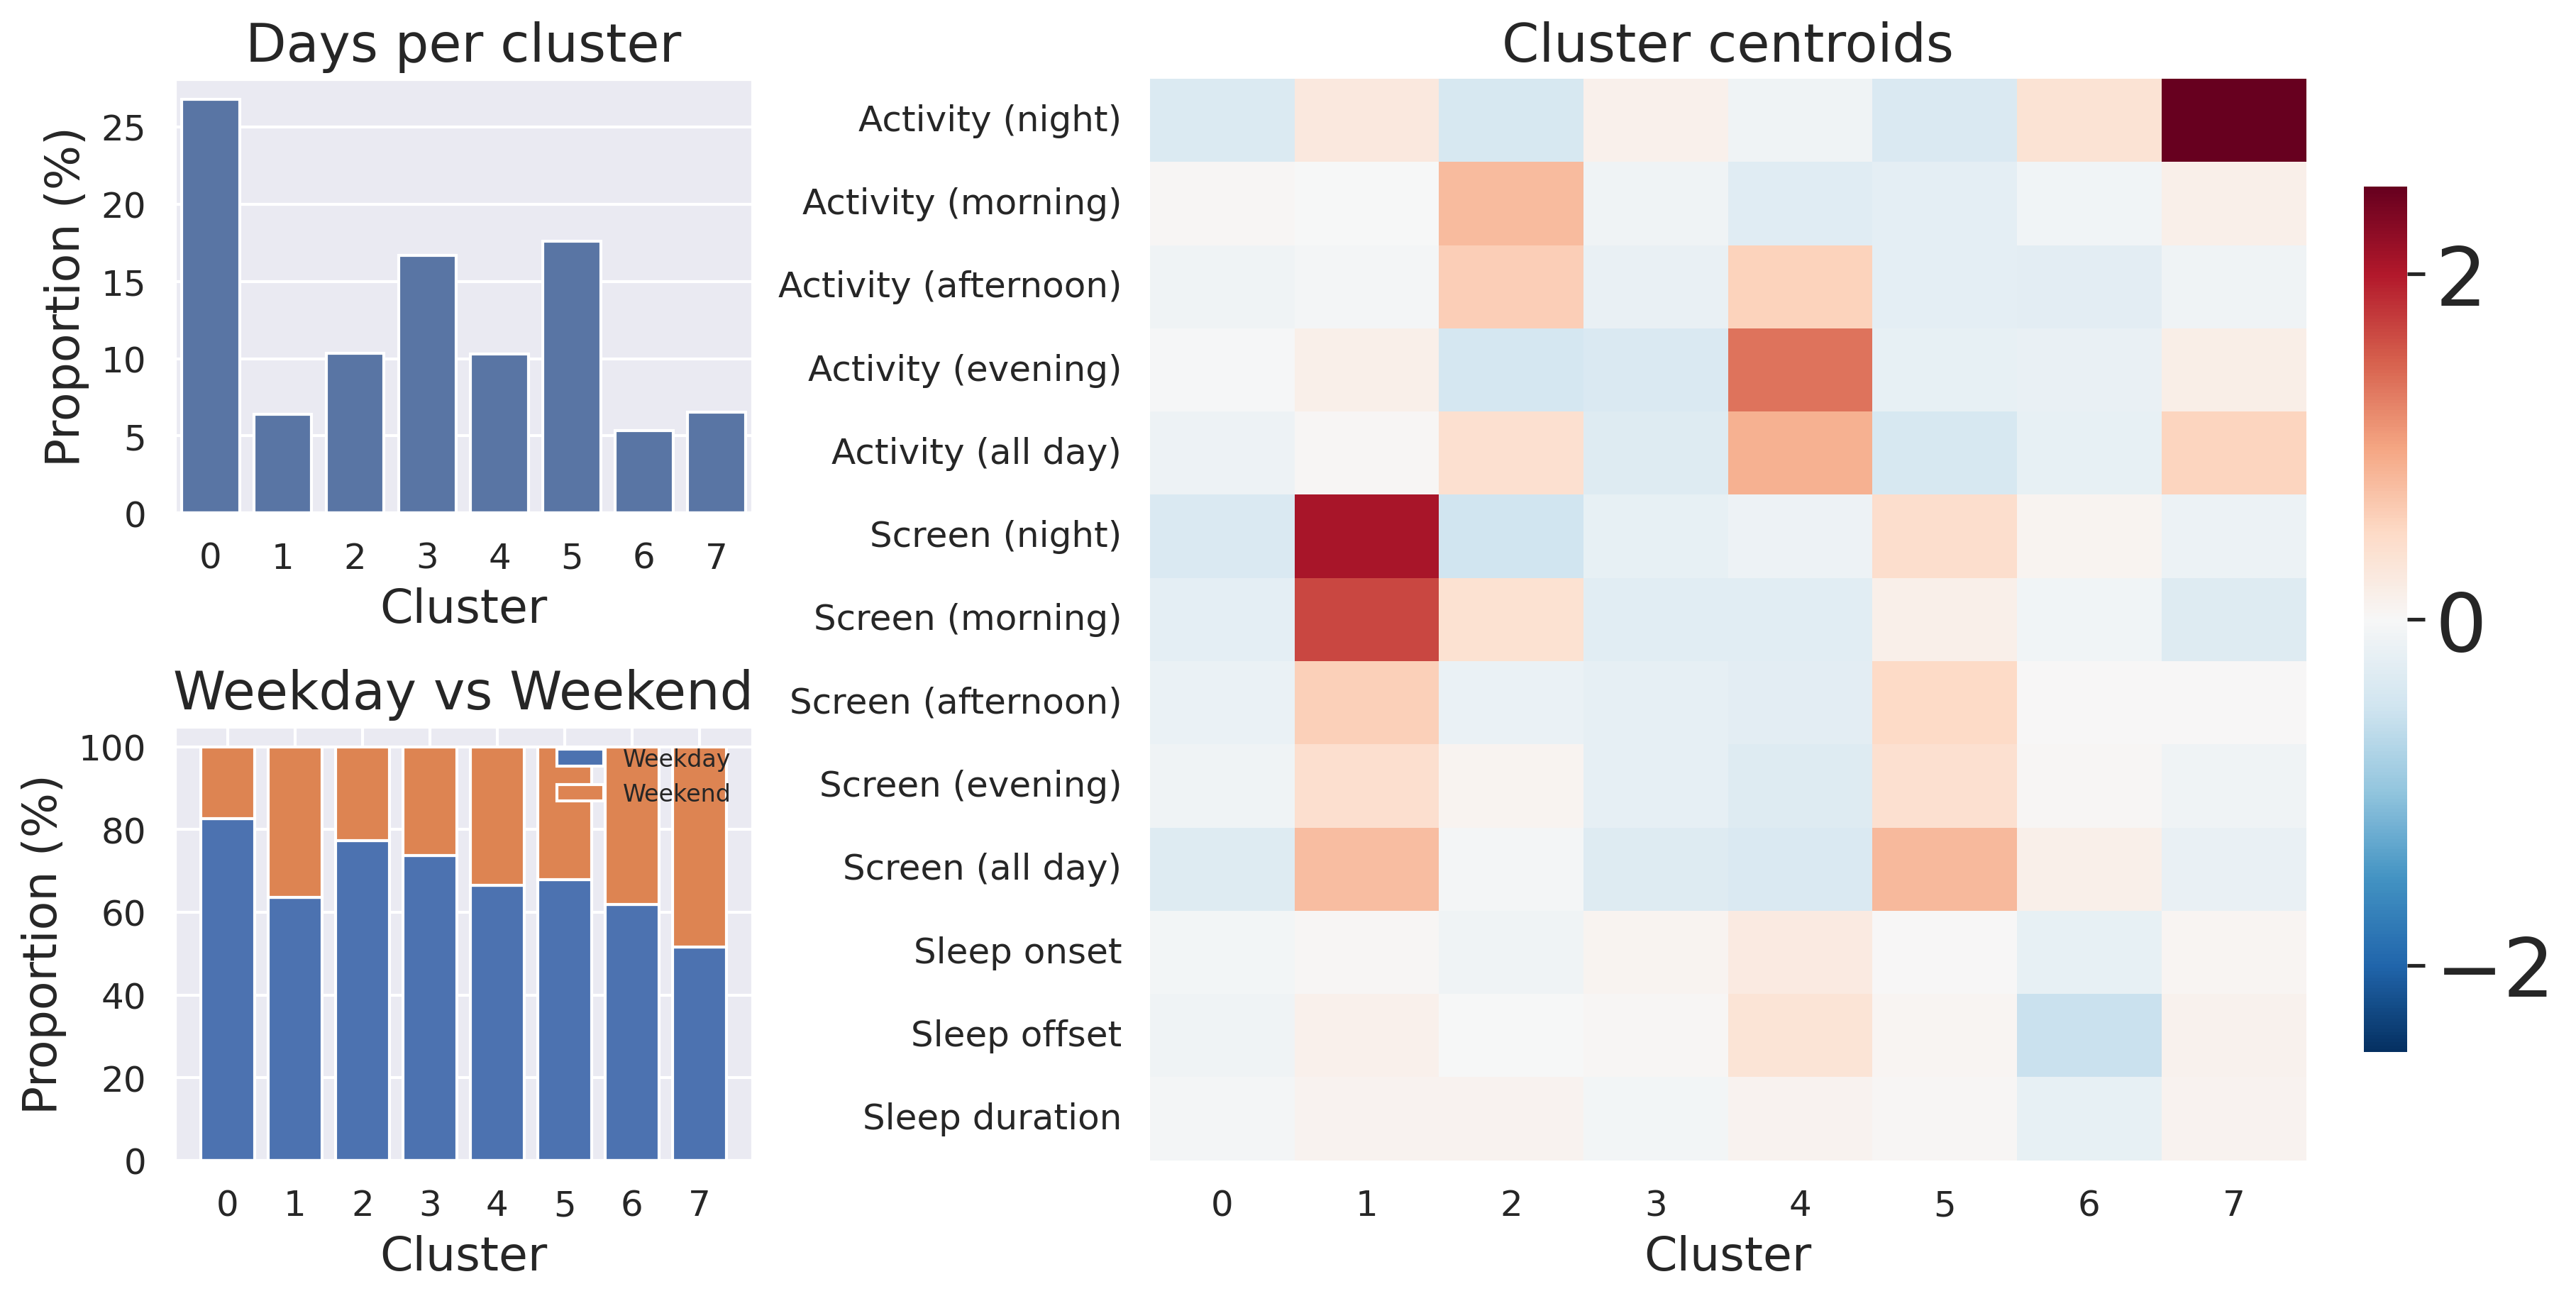
\includegraphics[width=\linewidth]{figures/appendix/globem_INS-W_2_summary.png}
    \caption{Cluster 2}
    \label{fig:globem_centroids_b}
  \end{subfigure}

  \medskip

  \begin{subfigure}[t]{0.485\textwidth}
    \centering
    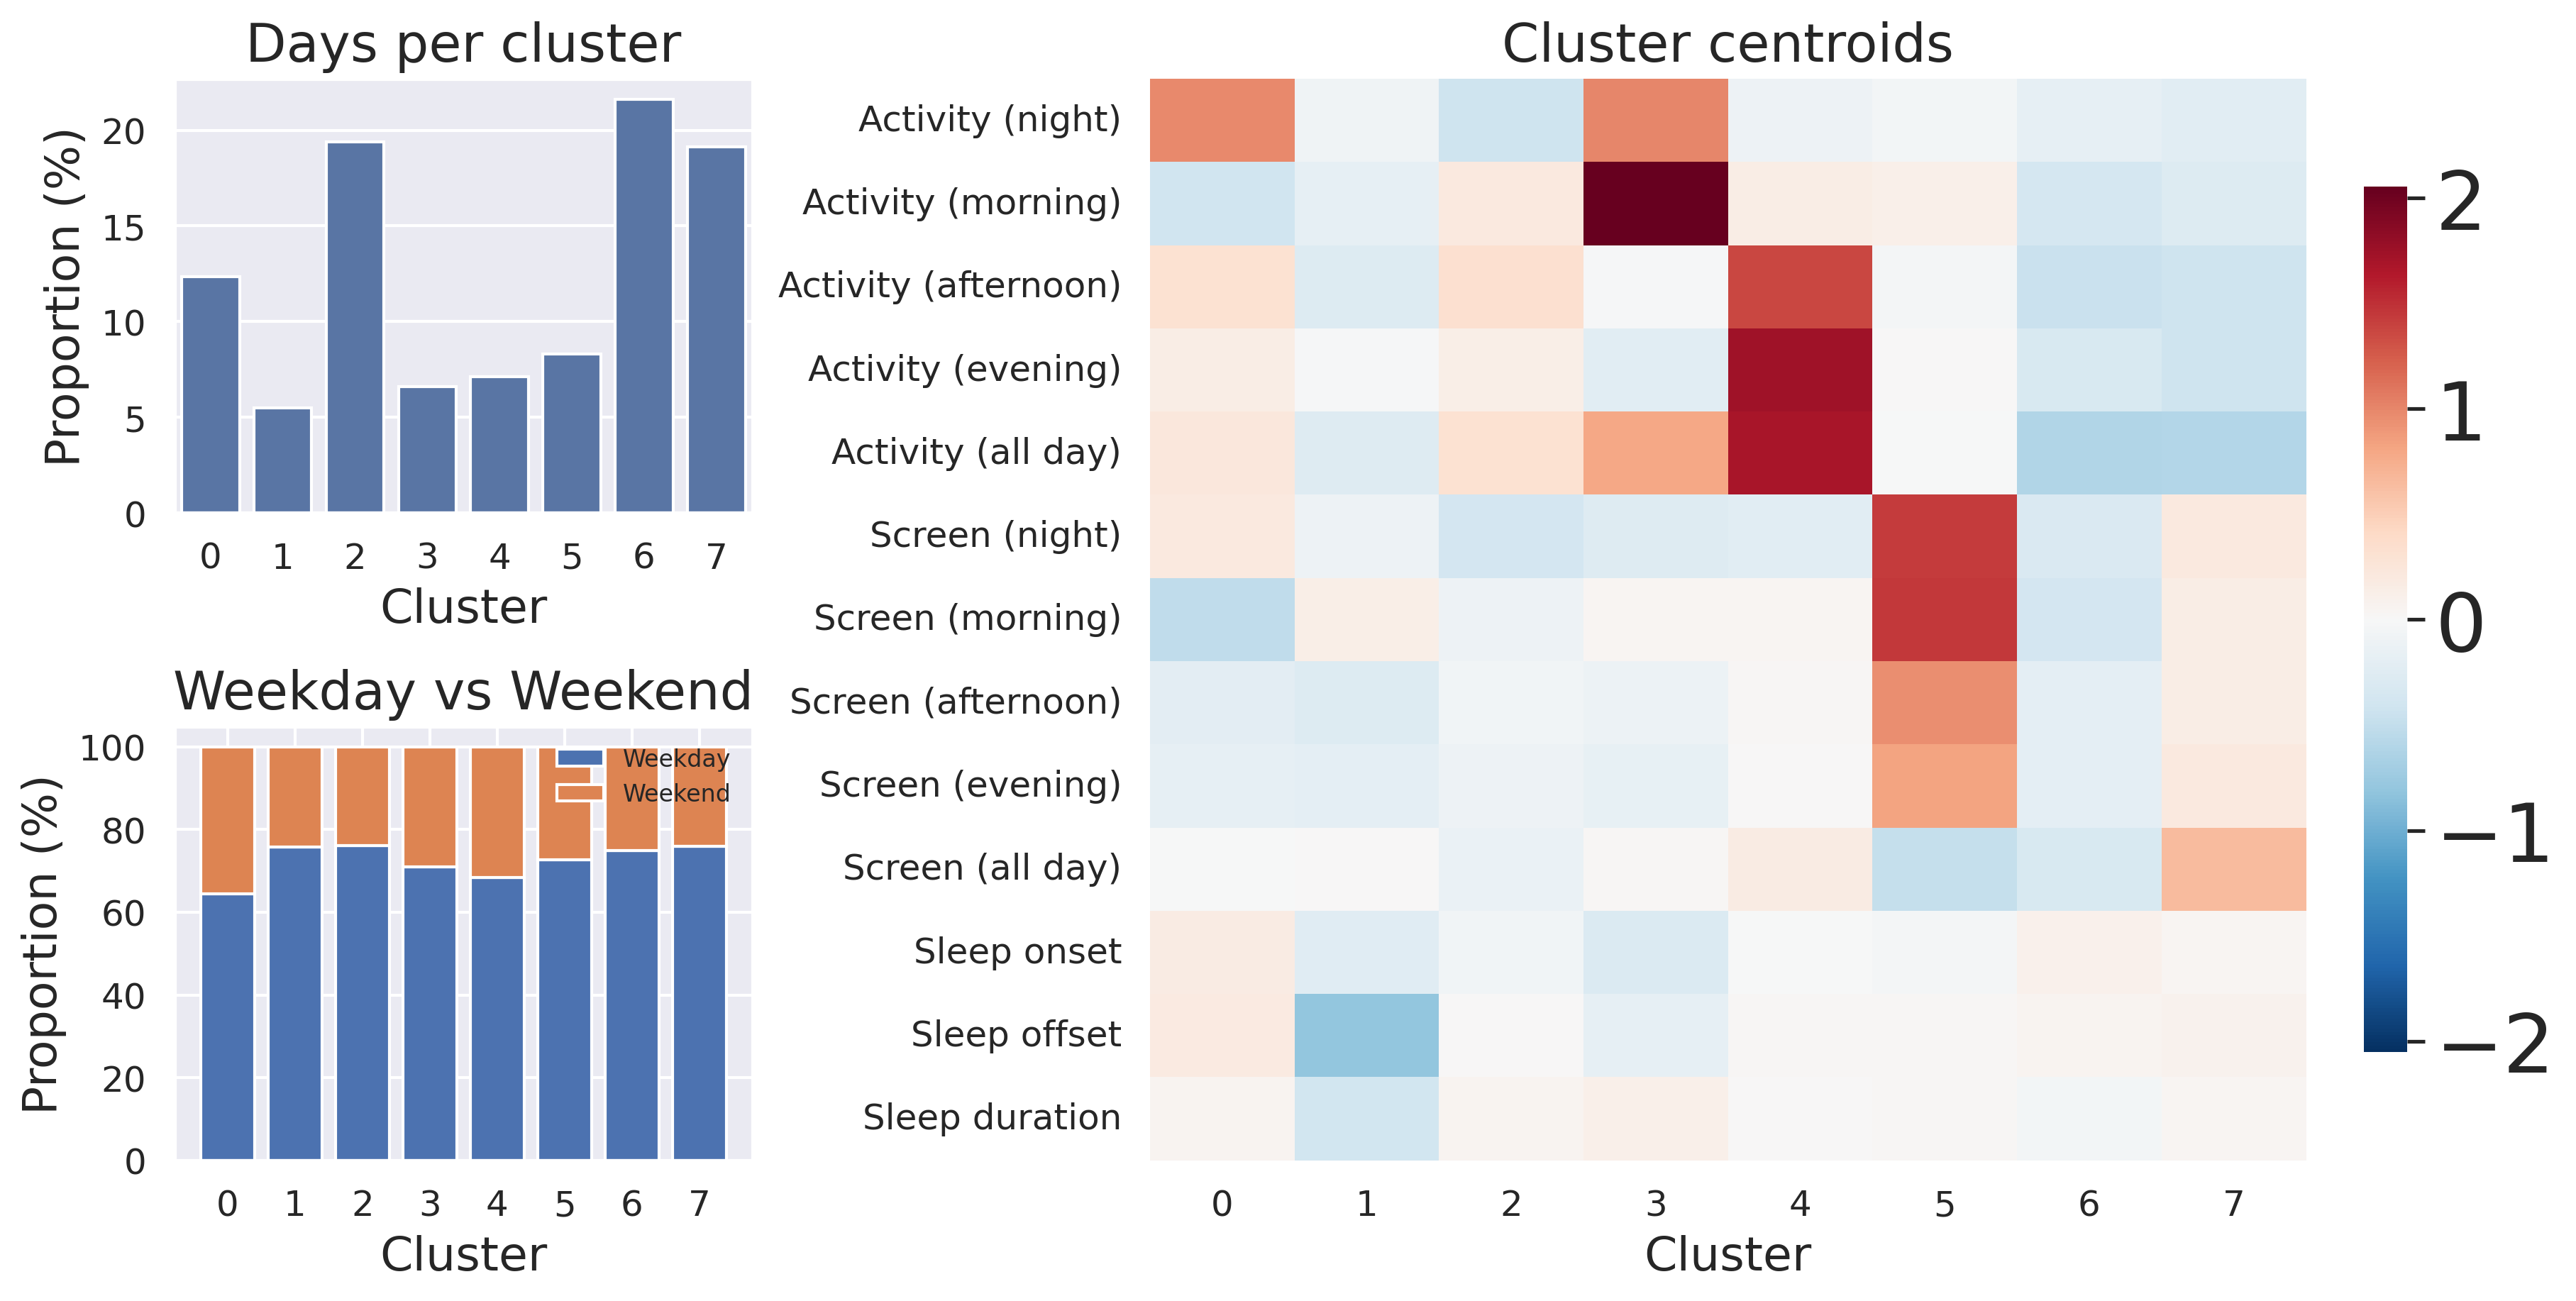
\includegraphics[width=\linewidth]{figures/appendix/globem_INS-W_3_summary.png}
    \caption{Cluster 3}
    \label{fig:globem_centroids_c}
  \end{subfigure}\hfill
  \begin{subfigure}[t]{0.485\textwidth}
    \centering
    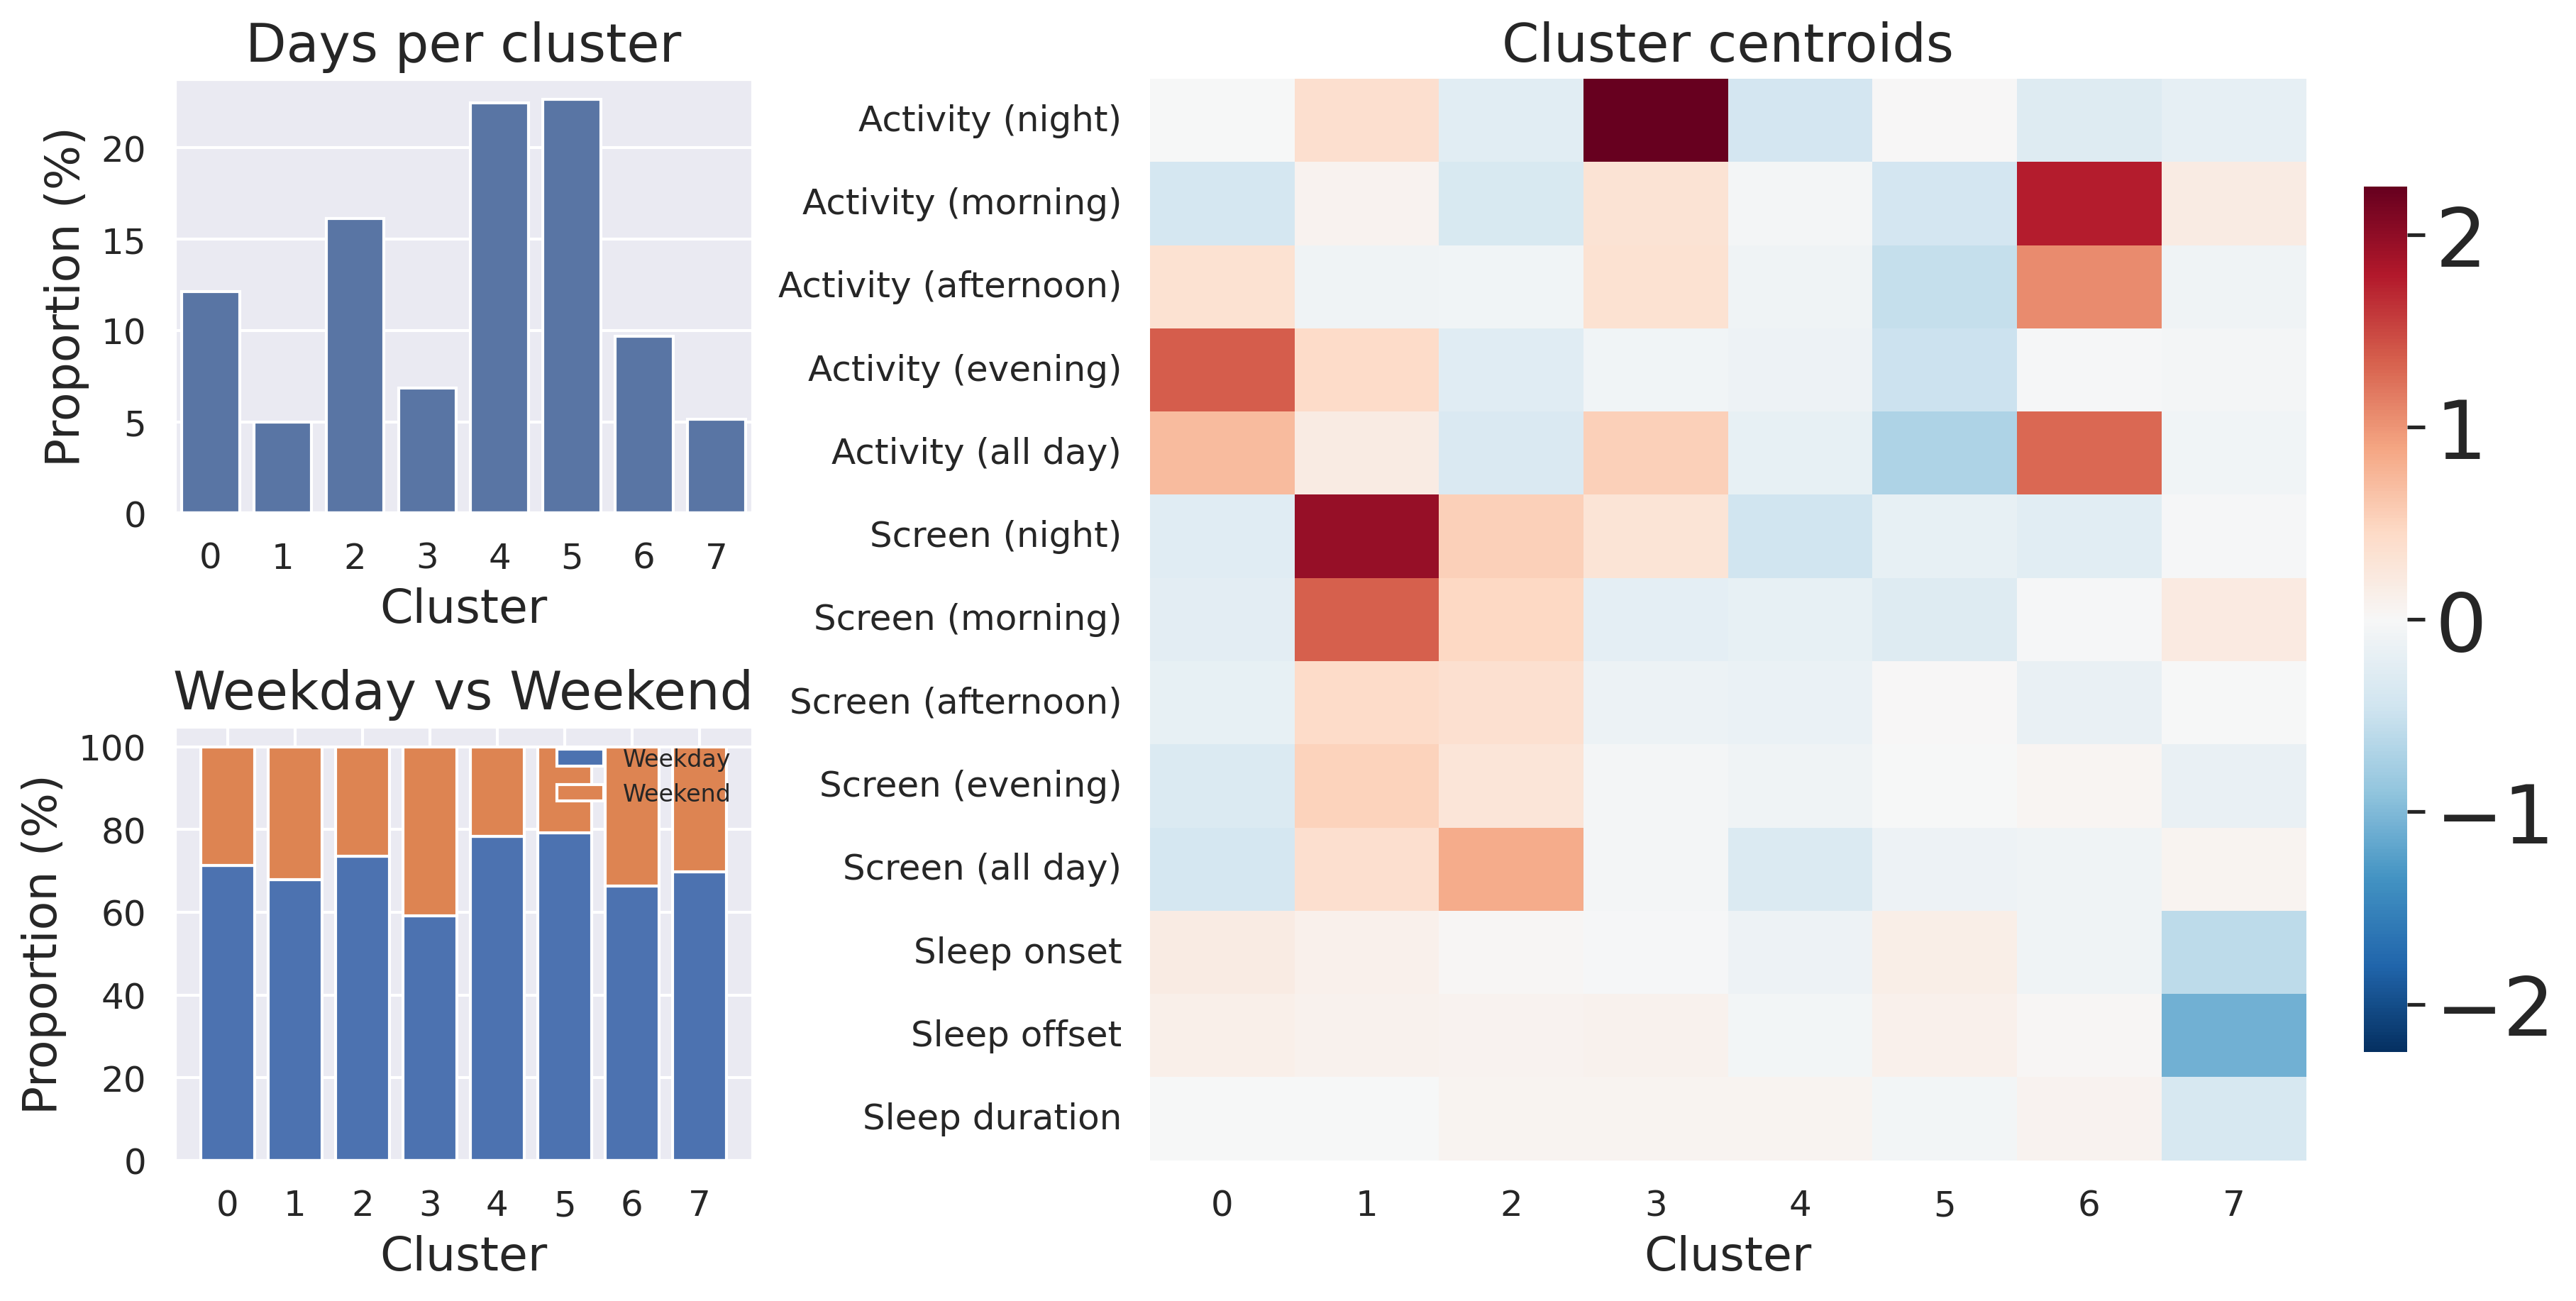
\includegraphics[width=\linewidth]{figures/appendix/globem_INS-W_4_summary.png}
    \caption{Cluster 4}
    \label{fig:globem_centroids_d}
  \end{subfigure}

  \caption{GLOBEM: Cluster centroid characteristics.}
  \label{fig:globem_centroids}
\end{figure}


% ---------- C: Signature with varying K ----------
\clearpage
\section{Signature with varying K components}

% (Add your figures/tables for this section here; using [p] + \FloatBarrier keeps them on this section’s pages.)

% \begin{figure}[p]
%   \centering
%   \includegraphics[width=\linewidth]{figures/appendix/signature_varying_K.png}
%   \caption{Signature stability under varying number of components K.}
%   \label{fig:signature_varying_K}
% \end{figure}
% \FloatBarrier

\end{appendices}


\end{document}
